\documentclass{article}

% if you need to pass options to natbib, use, e.g.:
% \PassOptionsToPackage{numbers, compress}{natbib}
% before loading nips_2016
%
% to avoid loading the natbib package, add option nonatbib:
% \usepackage[nonatbib]{nips_2016}

\PassOptionsToPackage{numbers,sort&compress}{natbib}
\usepackage[final]{nips_2016} % produce camera-ready copy

\usepackage[utf8]{inputenc} % allow utf-8 input
\usepackage[T1]{fontenc}    % use 8-bit T1 fonts
\usepackage{hyperref}       % hyperlinks
\usepackage{url}            % simple URL typesetting
\usepackage{booktabs}       % professional-quality tables
\usepackage{amsfonts}       % blackboard math symbols
\usepackage{nicefrac}       % compact symbols for 1/2, etc.
\usepackage{microtype}      % microtypography
\usepackage{graphicx}
\usepackage{float}
\usepackage{caption}
\usepackage{multirow}
\usepackage[labelformat=simple, labelsep=colon]{subcaption}
\renewcommand\thesubfigure{Figure ~\thefigure (\alph{subfigure})}
\title{A Clustering Based Music Recommendation System}

% The \author macro works with any number of authors. There are two
% commands used to separate the names and addresses of multiple
% authors: \And and \AND.
%
% Using \And between authors leaves it to LaTeX to determine where to
% break the lines. Using \AND forces a line break at that point. So,
% if LaTeX puts 3 of 4 authors names on the first line, and the last
% on the second line, try using \AND instead of \And before the third
% author name.

\author{
  s2569187\\
  %% examples of more authors
  \And
  s2511480\\
 \And
  s2594185\\
}

\begin{document}

\maketitle

\begin{abstract}

This report focuses on the task of using unsupervised techniques for clustering songs in the Spotify Dataset and leverages similarity between songs as a content-based filtering approach to build a Music Recommendation System. Data transformations are performed to extract relevant features from data and dimensionality reduction techniques help visualise the clustering results. The K-Means algorithm with six clusters achieved the best score on the Davies-Bouldin and Calinski-Harabasz indices. While Euclidean Distance proved to be a better metric to suggest similar tracks with respect to a single song, Cosine Similarity generated more accurate and diverse recommendations when a playlist was input to the system.

\end{abstract}

\section{Introduction}
The advent of digital music streaming platforms like Spotify, Amazon Music and Apple Music has resulted in a rapid growth in the volume of available music, making it increasingly challenging for users to discover new songs. A music recommendation system is ubiquitous due to its ability to ensure content discovery by narrowing down the plethora of available music to fit the unique tastes of a user. They play a pivotal role in enhancing user engagement, boosting revenue and driving business growth of organizations while significantly impacting audio experience of millions of people globally.

In recent literature, a content based recommendation system achieved 80\% Cosine similarity on Spotify data from 1921 - 2020 \cite{latex4e}. Velankar et al. \cite{latex6e} discussed content-based methodologies for feature identification in music analytics. Peng Liu et. al \cite{latex2e} discussed Pearson's correlation coefficient, Cosine, Chebyshev, Jaccard measures to calculate similarity or distance. P. Darshna offered a hybrid content-based and collaborative filtering approach. \cite{latex3e}. F. Fessahaye et al. proposed a deep learning based approach to address the Spotify RecSys 2018 Challenge \cite{latex1e}. Our dataset is fairly more recent (2017 - 2023) and we use clustering approaches to validate our content based recommendations.

In this report, we focus on exploring optimal methods for clustering unique songs in the dataset and use dimensionality reduction for visualizing the obtained clusters. We leverage these clusters and use similarity metrics to build a content-based recommender system that utilizes user input, taken in the form of both individual tracks and multiple songs, to curate personalized audio playlists for a user.

\section{Data Preparation}
The "Top 200" globally published playlists from 2017 to 2023 dataset by Spotify contains 651936 songs. We cleaned and pre-processed data by using a heatmap of column counts to check for missing values which, notably, were absent (\hyperref[app:heat-map]{Appendix A}). Since we aimed to build a recommendation system, we filtered out the 7457 unique songs and streamlined the dataset by grouping the duplicate entries for all the songs that featured multiple artists. Scatter plots for Loudness and Speechiness (\hyperref[app:outliers-scatterplot]{Appendix A}) confirmed the presence of very few outliers, which were retained as they represented natural variations in data and did not skew our results. Next, we focused on ensuring the quality of data by aggregating relevant features and dropping unnecessary columns like ‘date’, ‘id’, ‘Song URL', and other artist-related features as they do not affect the recommendation. The assignment of 'points' was contingent on the rank of a song, so we discarded it as song popularity is not relevant to our task.

It was necessary to engineer our features to feed them into a content-based filtering algorithm. Features like Loudness, Danceability, Energy, Speechiness, Acousticness, Instrumentalness and Valence were continuous valued and exhibited distinct ranges. Loudness encompassed unconstrained negative and positive values spanning into the thousands. This variability could potentially impact recommendation results, given that they rely on measuring the distance between data points. To mitigate this issue, all features were normalized to a range between 0 and 1 using the Min-Max Scaler 


\section{Exploratory Data Analysis}
Our EDA commenced with analyzing the descriptive statistics for the transformed dataset of 7457 songs and 7 features. Creating distribution plots like histograms, as shown in Figure 1, helped us understand the statistical distribution of song attributes by offering insights into the central tendencies, variability, and potential data clusters within features like danceability, energy, valence, and more.

Danceability and energy exhibited asymmetry, with one tail longer than the other. Both features gravitated towards higher values, indicating a prevalence of dance-friendly, energetically charged tracks. The histogram for Loudness showed a positively skewed, long-tailed distribution with two spikes signifying high-frequency occurrences of songs with a mean loudness of -5000. Acousticness and Speechiness followed a power-law distribution, indicating that most songs are electronically produced and have a fair balance between the vocals and instrumental sections. A spike at the lower end of the scale for Instrumentalness emphasized the overall dominance of tracks with vocals and lyrics over purely instrumental songs. Valence showed a concave distribution, suggesting that songs with highly positive or negative emotional content were rare. Additional EDA involved analyzing the feature distributions of the Top and Bottom 500 songs as seen in \hyperref[app:FEATURES500]{Appendix A}.

\begin{figure}[H]
    \centering
    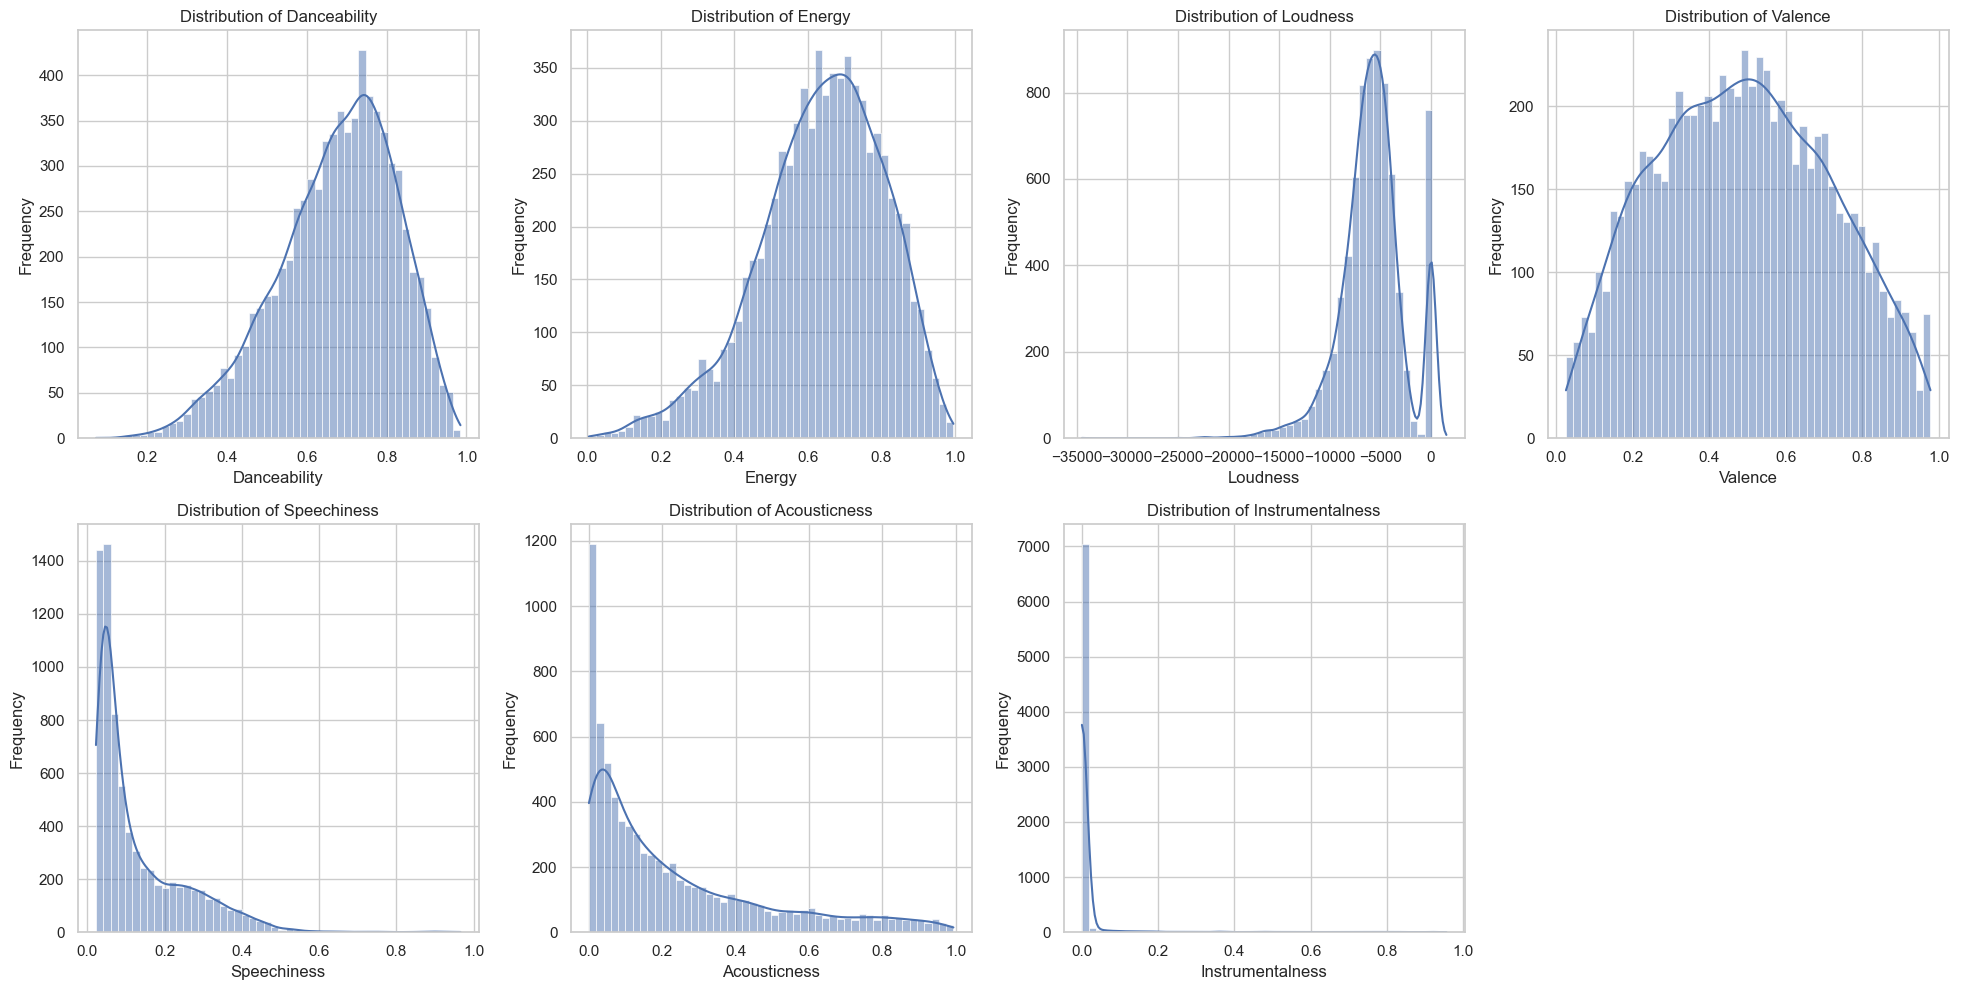
\includegraphics[width=0.73\linewidth]{Images/FeatureDistNew.png}
    \caption{Histograms to study the distributions of the continuous features in the dataset}
\end{figure}

\begin{figure}[H]
\centering
\begin{minipage}{.48\textwidth}
  \centering
  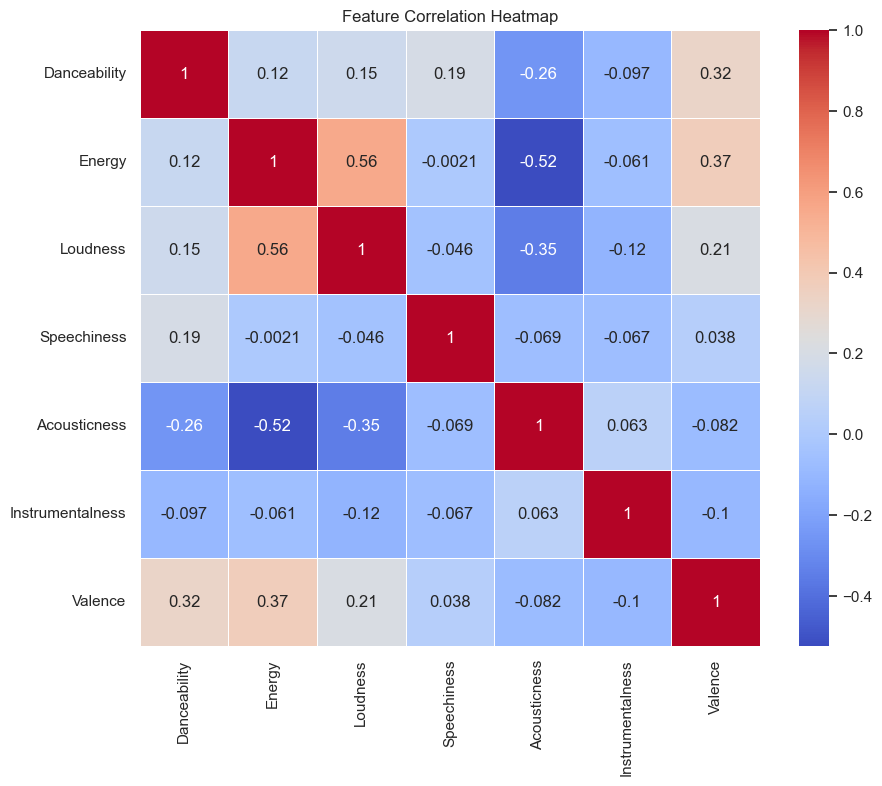
\includegraphics[width=40mm]{Images/Correlation HeatMap.png}
  \subcaption{Correlation Heatmap of features}
  \label{fig:testx}
\end{minipage}%
\begin{minipage}{.50\textwidth}
  \centering
  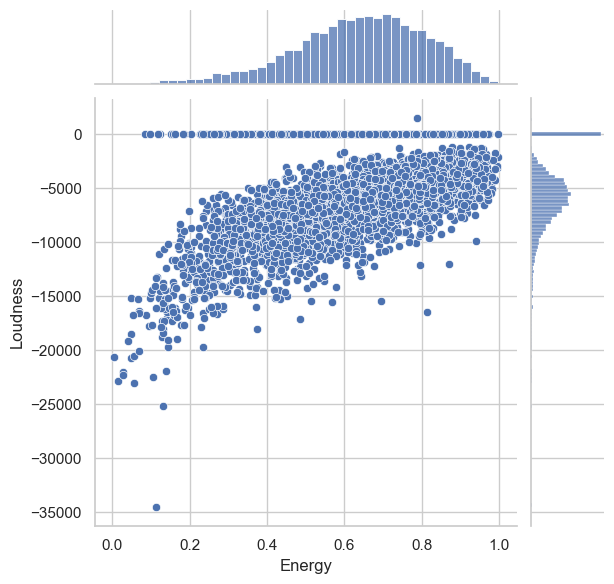
\includegraphics[width=37mm]{Images/Scatter Plott for Loudness and Energy.png}
  \subcaption{Loudness v/s Energy JointPlot}
  \label{fig:testy}
\end{minipage}
\end{figure}

The correlation Heatmap shown in Figure 2(a) revealed that most features exhibited low to moderate correlations, with values generally below 0.5, suggesting weak linear relationships between them. However, loudness and energy demonstrated a relatively stronger positive correlation, indicating that loud songs often had higher energy associated with them. Figure 2(b) shows a joint plot to visualise this observation and confirms a definitive correlation between this pair of features.


\section{Learning Methods}
\subsection{Clustering}

We train the dataset to group the transformed data comprising 7457 songs into their respective clusters and visualise them in 2D and 3D space using PCA and t-SNE. Density-based DBSCAN clustering\cite{latex9e}, centroid-based K-Means clustering and hierarchical methods like Agglomerative clustering\cite{latex8e} have been implemented and evaluated using intrinsic metrics to determine the best algorithm.

\subsubsection{Density-Based Spatial Clustering}
Our implementation of DBSCAN required us to tune a hyper-parameter, epsilon, by heuristically detecting a knee-point in a k-distance graph, constructed using the Nearest Neighbors approach (\hyperref[app:DBSCAN]{Appendix B}). After visualizing the cluster using PCA, it was observed that even with optimal hyper-parameters it produced only one cluster with noise, possibly due to varied densities of clusters for the given data. We rejected DBSCAN and further explored centroid-based algorithms for clustering.

\subsubsection{Centroid Based Clustering}

To ascertain the optimal number of clusters in centroid-based clustering, we plotted the sum of the squared distance between cluster points and centroids against different values of K ranging from 2 to 20. Using the elbow method shown in Figure 3(a), we identified a point of diminishing return having the steepest gradient at K = 6. Beyond this, increasing k did not significantly reduce the within-cluster sum of square distances. A more rigorous Silhouette analysis confirmed that the heuristically chosen value of K (= 6) was indeed optimal for producing highly distinguishable clusters.

We used K-Means clustering, which recursively selects a centroid for each cluster and categorizes a data point into a cluster based on its distance from the centroid. Starting with 6 clusters, we set a high value for n\_iter (= 100) and a low value for tolerance (= 0.0001) so that the algorithm scans the entire feature space to choose the most stable clusters. Instead of randomly initializing the centroids, we used kMeans++ for faster and better convergence to more consistent and globally optimum clusters. 

\begin{figure}[H]
\centering
\begin{minipage}{.6\textwidth}
  \centering
  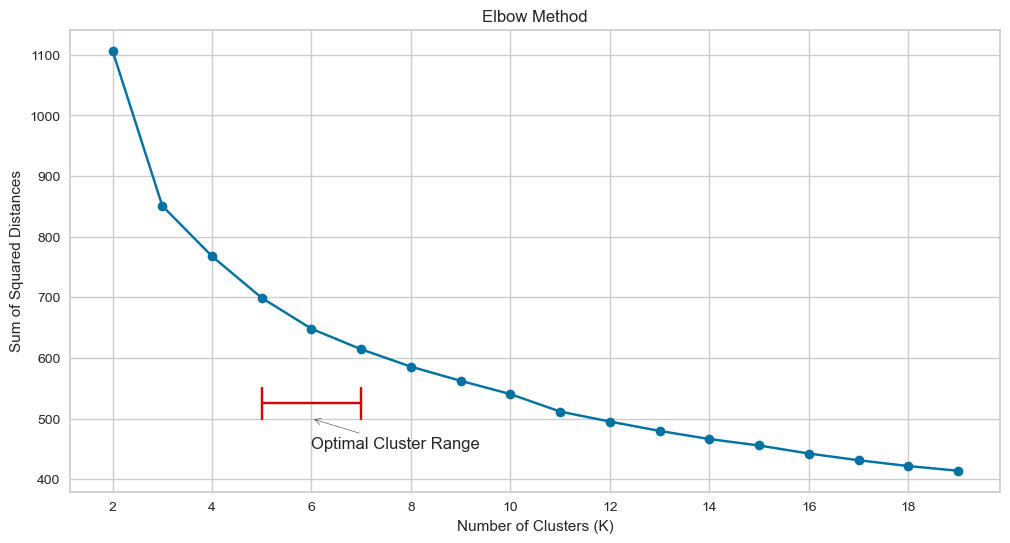
\includegraphics[width=70mm]{Images/CLUSTER K EBLOW.png}
  \subcaption{Elbow plot to find optimal K}
  \label{fig:test3}
\end{minipage}%
\begin{minipage}{.4\textwidth}
  \centering
  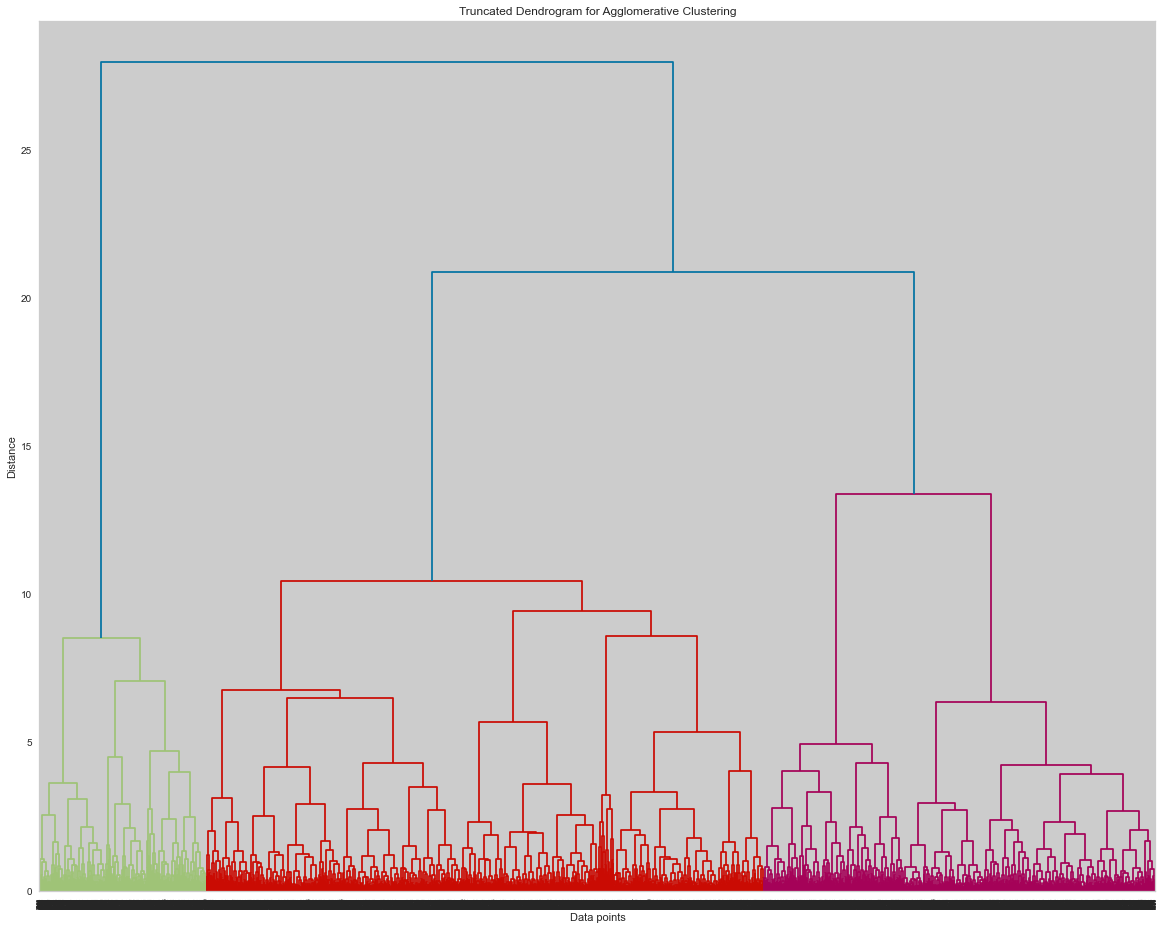
\includegraphics[width=43mm]{Images/WARD.PNG}
  \subcaption{Dendogram - Ward's linkage}
  \label{fig:test4}
\end{minipage}
\end{figure}


\subsubsection{Hierarchical Clustering}

An alternate approach like Hierarchical Agglomerative Clustering was used to cluster data without an apriori determination of the number of clusters. We analyzed the resulting Dendrograms created using single, complete, and Ward's linkages to interpret how songs were grouped based on their relationships with their attributes. The dendogram for Ward's linkage shown in Figure 3(b), exhibited a gradual and structured merging of four equally sized clusters with lower cluster fusion heights with denser and longer branching patterns, indicating higher intra-cluster homogeneity and greater inter-cluster separation compared to the dendogram for complete linkage (\hyperref[app:completeLink]{Appendix C}).

% For BIRCH, we used a default branching factor of 50 and experimented with multiple threshold values [0.5, 5], to obtain 18 optimal clusters at the threshold value of 2.5. The visualisation of BIRCH is in \hyperref[app:birch_pca]{Appendix C}

% \subsubsection{UMAP}
% To preserve both local and global structures in data by prioritising both, intra and inter-cluster distances, we used UMAP to find the projection of each track in its respective cluster by separating these groups of similar categories much more clearly for better visualisation. The balance between local and global structure in the final projection was achieved by optimising values for the parameters n\_neighbors and min\_dist and analysing their impact on the resulting projection.

% As our application of UMAP is primarily for visualization purposes, we opted not to employ specific metrics for calculation. Instead, we conducted iterations over the parameters n\_neighbors and min\_dist across a range of values, specifically within the intervals [1-100] and [100] respectively. Through this exploration, we identified that the visualizations were more satisfactory when these parameter values were at n = and dist =. Refer to \hyperref[app:UMAP]{Appendix E} for plots of UMAP for various sets of parameters.

\subsection{Visualization}
The dataset is engineered to focus on 7 continuous-valued features. The objective of visualisation was to determine where a particular track is located in a cluster, relative to other songs, by projecting its position onto lower dimensions. Abiding by the manifold hypothesis, we reduced the dimensionality of the dataset using techniques like PCA and T-SNE to visualise it in 2 and 3 dimensions.

\subsubsection{Principal Component Analysis}
PCA is a linear dimensionality reduction technique that we employed to visualise our 7-D data in a 2-D space before and after clustering as illustrated in Figure 4. Scaling the features ensured that the principal component vectors did not get skewed due to differences in scale. It is evident from the figure that 90\% of the cumulative variance is explained by five PCs. The explained variance ratios after projection are 41.53\%, 26.40\%, and 12.32\% for PC1, PC2, and PC3 respectively (\hyperref[app:expVariance]{Appendix D}). PCA, however, assumes the linear relationship between features and concerns itself only with the global (inter-cluster) structure of data.

\begin{figure}[h]
\centering
\begin{minipage}{.35\textwidth}
  \centering
  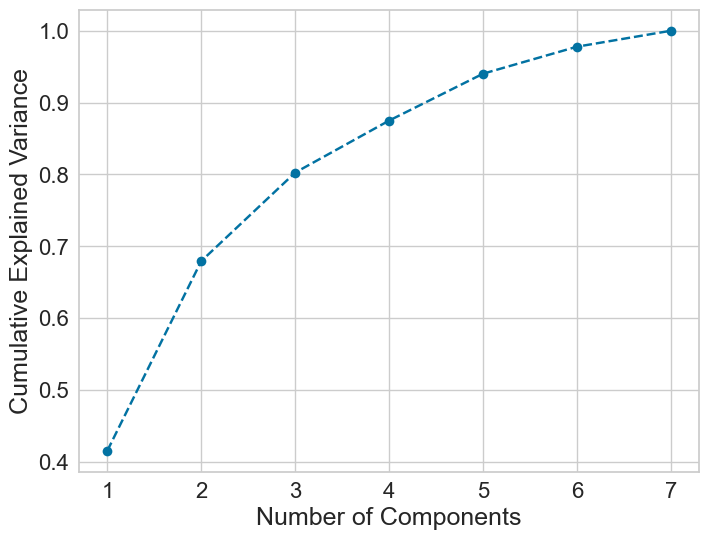
\includegraphics[width=45mm]{Images/CUM VARIANCE.png}
  \label{fig:tdassS}
\end{minipage}%
\begin{minipage}{.65\textwidth}
  \centering
  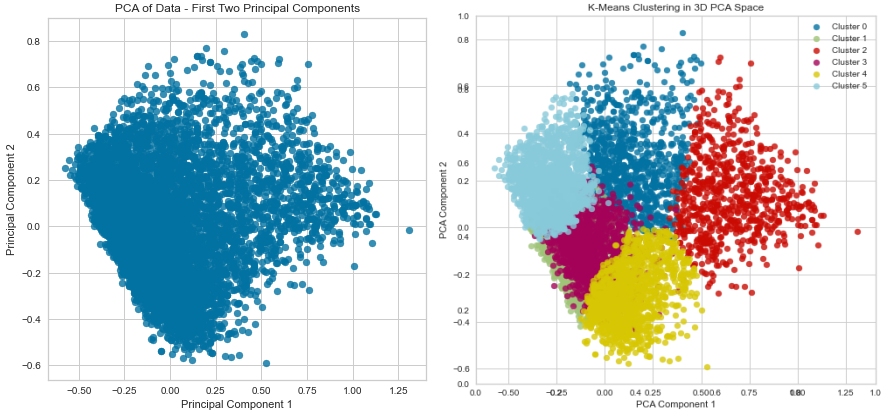
\includegraphics[width=77mm]{Images/K-meansBeforeAfter.png}
  \label{fig:aDDF}
\end{minipage}
\caption{Cumulative Variance explained by the Principal Components for the transformed data and its 2-dimensional visualisation with and without cluster labels. The 3D visualisation is in \hyperref[app:kmeans_pca]{Appendix D}}
\end{figure}

\subsubsection{t-distributed Stochastic Neighbourhood Embedding}
 Unlike PCA, T-SNE, an unsupervised, non-linear dimensionality reduction technique for high-dimensional data visualisation preserves the local (intra-cluster) structure of data \cite{latex7e}. The optimal value of the parameter epsilon was set to 14, twice the number of dimensions in our data \cite{latex5e}. The hyper-parameter perplexity was calculated by plotting the KL Divergence  over a range of perplexity values from 1 to 100, iterating in steps of 3 to alleviate the computational load. We observed that the metric stabilized after reaching a perplexity of 80, resulting in more consistent clusters (\hyperref[app:TSNEPerp]{Appendix E}).

\subsection{Recommendation System}

%Content-based recommender systems tailor recommendations to users by analyzing the intrinsic characteristics and attributes of items and mapping them to user preferences. %In the context of Spotify's data, we measure the utility of content-based filtering through similarity heuristics to measure the likeness between the user's recently played song and other songs in our dataset. This enables us to make relevant recommendations, thus enriching and enhancing the user experience.

For our recommendation system, we initially considered a baseline model using the Pandas corrwith() function to compute the pairwise Pearson Correlation Coefficient for each song against all others in the data. Low correlation values among features conveyed that this baseline model failed to capture the complex non-linear relationships between songs. Consequently, we decided to forego this method and opted for more advanced content-based filtering algorithms which provided a more nuanced understanding of the item-item similarity between songs to facilitate more accurate recommendations.

The knowledge that each cluster has similar music in it served as a hard boundary for us to leverage similarity metrics like Manhattan and Euclidean distance for recommending songs. It circumvented the risk of recommending music unrelated to a user’s taste. Based on the minimum distance between the feature vectors, the model searched for the "closest" songs that were represented by similar feature values as the input song. More similar songs ranked higher on the recommendation list. However, our feature vectors comprised of numerical values, and considering their magnitude may cause the sum of squared differences to assume very large values, thus skewing our recommendation. To mitigate this, we considered a recommendation model using an alternate distance metric known as cosine similarity which captured directional relationships between feature vectors rather than magnitudes alone. By computing the normalized dot product of the two 1 x 7 feature vectors, we obtained the values of cosine similarity which varied between [-1, 1]. A higher value of cosine similarity implied greater likeness between two songs and thus a more likely recommendation.

% These clusters can guide the recommendation systems to suggest tracks that align with users' preferences. If a user tends to prefer high-energy, danceable songs with low acoustic elements and high valence, the system can suggest tracks from clusters that match these preferences.

A comprehensive evaluation of the performance of our recommendation system was conducted by considering two distinct user types. To assess the system's ability to make effective recommendations for focused audio choices, User 1 submitted a single song as input and sought the Top 5 most relevant recommendations. Meanwhile, User 2 provided a playlist of songs as input, reflecting a broader set of preferences and diverse musical tastes. Considering both types of users allowed for the examination of the system's behaviour across different absolute values and ranges of feature values.

% Cosine similarity was chosen as a metric because of its compatibility with techniques like PCA and t-SNE and its robustness irrespective of the scale of data. By measuring similarity in terms of angle rather than distance, we reduce the dimensions of the vectors without significantly affecting the cosine similarity measure.

%We loaded the feature values of the user’s chosen track or playlist in one data frame and populated another with the features of all other 7457 songs in our dataset, passing them as input parameters to the cosine similarity function. We iterate over the data frames to compute the cosine similarity between our input and each of the other songs and append the resulting values into a new column, sorted in descending order of cosine similarity, to predict similar songs which the user is most likely to hear.

\section{Results and Discussion}

\subsection{Clustering and Visualization}

To identify the most effective clustering technique, a comprehensive evaluation was conducted using three intrinsic metrics. From Table 1, it was evident that K-Means was the optimal clustering method, achieving the minimum Davies-Bouldin value while concurrently attaining the highest Silhouette and Calinski-Harabasz scores. On visualising the clusters using dimensionality reduction techniques, we observed minimal variance in the Davies-Bouldin index. However, the Calinski-Harabasz index using t-SNE resulted in significantly higher values than PCA, with K-means clustering attaining the highest score of 2046. Agglomerative Clustering scored around 1600 on this index, proving that overall, t-SNE resulted in more distinguishable and denser clusters than PCA. The better clustering method, K-Means, when projected using t-SNE, showed optimal cluster separation and cohesion (Figure 5).

\begin{figure}[H]
\centering
\begin{minipage}{.5\textwidth}
  \centering
  %\begin{table}
  \resizebox{70mm}{!}{%
\begin{tabular}{l c c}
\toprule
& \multicolumn{2}{c}{\textbf{Clustering Techniques}} \\
\cmidrule(l){2-3}
\textbf{Metrics} & \textbf{K-Means} & \textbf{Agglomerative} \\
\midrule
Silhouette & 0.1895 & 0.1308\\
Davies-Bouldin & 1.4112 & 1.7658\\ 
Calinski-Harabasz & 2046.13 & 1608.0266\\ 
\bottomrule
\end{tabular}
}
\captionof{table}{Evaluating Clustering Algorithms}
\label{tab:sadassdasaa}
%\end{table}
\end{minipage}%
\begin{minipage}{.5\textwidth}
  \centering
  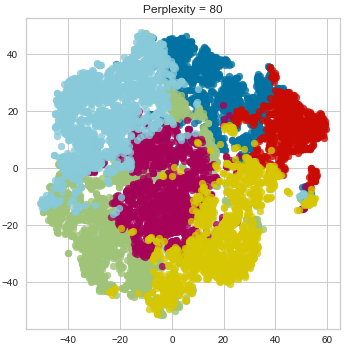
\includegraphics[width=39mm]{Images/t-SNE Kmeans.png}
  \caption{K-means Visualisation - t-SNE}
  \label{fig:SSASAX}
\end{minipage}
\end{figure}

\subsection{Cluster Profiling and Analysis}

Knowing that our data could be optimally grouped into 6 distinct clusters, we analysed each cluster to identify the types of songs in them based on the mean values of their seven features (Table 2). Cluster 0 had very natural and acoustic songs, with engaging and positive lyrics and diverse emotional essence. The songs in Cluster 1 had high energy and loudness with a good blend of vocals and music. Cluster 2 contained songs that were soft and soothing, composed of acoustics and instrumentals but the lyrics seem to be on the less happy side. Songs belonging to Cluster 3 were loud, energizing and positive in expression. They were mostly lyrical, like rap, and induced a lively atmosphere, conducive for dancing. Cluster 4 contained energetic songs with high beats but gloomy lyrics and had fewer acoustics and instrumentals. Danceable, loud and high-energy tracks with minimal instrumentals were found in Cluster 5. These songs too, had lyrics that invoked highly positive emotions. 

From Table 2, it was evident that Speechiness was highly dominant in Cluster 3, while Acousticness and Instrumentalness were very dominant in Cluster 2. This observed dominance was substantiated by examining the mean values of the features (\hyperref[app:Cluster_profile]{Appendix F}). The values of the other four features, namely Danceability, Loudness, Energy and Valence were more evenly distributed across the remaining clusters. The idea behind cluster profiling was that when we extended our project to build a recommendation system to suggest tracks that aligned with user preferences, these clusters would serve as a qualitative metric to evaluate our model’s recommendation. If a user preferred high-energy, danceable songs with low acoustic elements and high valence, the system must suggest tracks from clusters whose mean feature values matched the attributes of the preferred input song.

\begin{table} [H]
\centering
\resizebox{120mm}{!}{%
\begin{tabular}{c c c c c c c c}
\toprule
{C} & {Danceability}  & {Energy}  & {Loudness}  & {Speechiness}  & {Acoustic}  & {Instrumentalness}  & {Valence} \\
\midrule
0 & 0.6859 & 0.6089 & 0.7931 & 0.1253 & 0.5150 & 0.0118 & 0.6113\\
1 & 0.5937 & 0.7747 & 0.8346 & 0.0878 & 0.0877 & 0.0137 & 0.4834\\
2 & 0.4813 & 0.3469 & 0.6904 & 0.0677 & 0.7631 & 0.0437 & 0.2811\\
3 & 0.8034 & 0.5762 & 0.7807 & 0.2213 & 0.1073 & 0.0070 & 0.4165\\
4 & 0.5668 & 0.5971 & 0.7885 & 0.0783 & 0.1530 & 0.0202 & 0.1982\\
5 & 0.7476 & 0.7404 & 0.8302 & 0.1047 & 0.1334 & 0.0071 & 0.7803\\

\bottomrule 
\end{tabular}
}
\\[1ex]
\caption{Cluster Profiling using the mean values of features for each cluster} 
\label{tab:template1}
\end{table}

% We projected the clusters using dimensionality reduction techniques PCA and t-SNE to visualise them. We fit TSNE and transform the data using the value of epsilon and perplexity as found in section 4.2.2 and plot it using a Scatterplot to visualise the data Refer to \hyperref[app:TSNE]{Appendix D} for t-SNE plots with various perplexity values.  strong local clustering and grouped songs having similar feature values together.

\subsection{Recommendation System}

\begin{table} [ht]
\resizebox{\textwidth}{!}{%
% \centering

\begin{tabular}{l l l}
\toprule

\textbf{Manhattan Distance} & \textbf{Euclidean Distance} & \textbf{Cosine Similarity}\\
\midrule
Slide (feat. Frank Ocean \& Migo) \textbf{[0]} & Slide (feat. Frank Ocean \& Migo) \textbf{[0]} & Keii \textbf{[0]}\\ 
Morad: Bzrp Music Sessions. Vol. 47 \textbf{[0]} & Morad: Bzrp Music Sessions. Vol. 47 \textbf{[0]} & Reggaetonera \textbf{[0]}\\ 
Reggaetonera \textbf{[0]} & Reggaetonera \textbf{[0]} & Kids Again \textbf{[0]}\\ 
Poquito \textbf{[0]} & Poquito \textbf{[0]} & Fràgil \textbf{[1]}\\ 
Keii \textbf{[0]} & Keii \textbf{[0]} & Slide (feat. Frank Ocean \& Migo) \textbf{[0]}\\
\bottomrule
\end{tabular}
}
\\[1ex]
\caption{Recommendations for User 1. Cluster numbers mentioned in '[]' after song title}
\label{tab:template2}
\end{table}

While assessing the recommended tracks for User 1's randomly generated input song "All Around The World (La La La)", a notable consistency was observed across the three similarity metrics as a majority of the recommended songs (14/15) belonged to the same cluster as the input track (Cluster 0). Comparisons of mean feature values between user input and recommended songs (\hyperref[app:RECOM_MEAN_PLOT]{{Appendix G}}) unveiled substantial similarities among five attributes, demonstrating the robustness of the system. The fact that both Euclidean and Manhattan distance methods yield the same set of recommended songs for User 1 suggested a consistent outcome across the two distance metrics. 

\begin{table} [ht]
\resizebox{\textwidth}{!}{%
% \centering

\begin{tabular}{l l l}
\toprule

\textbf{Manhattan Distance} & \textbf{Euclidean Distance} & \textbf{Cosine Similarity}\\
\midrule
The Bones \textbf{[4]} & Yonaguni \textbf{[1]} & The Mantra (with Pharrell \& Kendrick Lamar) \textbf{[1]}\\ 
In My Head \textbf{[4]} & Never Leave Me (feat. Joe Janiak) \textbf{[1]} & Sexo Virtual \textbf{[1]}\\ 
Rich \& Sad \textbf{[4]} & I Don't Do Drugs (feat. Ariana Grande) \textbf{[1]} & Yonaguni \textbf{[1]}\\ 
Two of Us \textbf{[4]} & Panini \textbf{[0]} & Amantes y Amigos \textbf{[0]}\\ 
I Miss You (feat. Julia Michaels) \textbf{[4]} & Matt Hardy 999 (feat. Juice WRLD) \textbf{[1]} & CENERE\textbf{[4]}\\
\bottomrule
\end{tabular}
}
\\[1ex]
\caption{Recommendations for User 2. Cluster numbers mentioned in '[]' after song title}
\label{tab:template3}
\end{table}

User 2's input was a randomly generated playlist comprising of ten songs from different clusters \hyperref[app:RecSysOP]{{Appendix H}}. The use of Cosine Similarity effectively addressed the limitation of recommending tracks only from the same cluster as the input song. Mean value analysis underscored the proficiency of this metric in recommending songs as the attribute values of the recommended tracks were comparable to the mean characteristics of the input songs across six features in \hyperref[app:RecSysOP]{{Appendix H}}. As seen in Table 4, the recommendations spanned a wide range of clusters emphasizing the robustness of the system in capturing accurate user preferences compared to other distance methods.

Despite the overall success of the system, we identified discrepancies in the mean values of speechiness and instrumentalness, suggesting potential areas for improvement and highlighting the challenges in optimizing recommendation systems. These disparities could be attributed to the skewed power law distribution of these features. Understanding the impact of skewed data on these features is crucial for algorithm refinement and exploring strategies such as re-weighting could prove beneficial.



\section{Conclusion}

The K-Means algorithm with 6 centroids was found to be the best technique for clustering the 7497 unique songs, scoring the lowest on the Davies-Bouldin index and attaining the highest values for the Silhouette and Calinski-Harabasz metrics. On visualising the resulting clusters using dimensionality reduction techniques, K-Means with t-SNE was observed to depict maximum homogeneity and most distinct cluster separation. Analysis of the cluster profiles revealed the type of songs in each cluster.

While building our content-based recommendation system, content based filtering approaches like Manhattan, Euclidean and Cosine Similarity helped us outperform the naïve correlation-based recommendation baseline. For recommendations based on a single input song, distance metrics tend to perform well because the distances between the feature values of a single input are more likely to be shorter, making the system suggest songs from the same cluster. Cosine Similarity, however, diversified song suggestions by capturing directional relationships rather than distance magnitudes alone, alleviating the hard boundary cluster constraints observed in single-input scenarios. It is more reflective of real-world scenarios where users have diverse preferences and evolving tastes. In the absence of extrinsic measures like user ratings, mean value analysis quantified the effectiveness of the system, while the balance between accuracy and diversity in the track recommendations qualitatively underlined its efficacy. 

\bibliography{refs.bib}
\bibliographystyle{plain}
\clearpage

\section*{Contributions} 
Each of the three authors contributed equally towards implementation of the code for this mini-project as well as writing the academic report about it. Feedback of each individual was valued equally and debated upon before finalizing the content of any section in the report.
\subsection*{1. s2569187}
Contributed towards preparing the data and engineering the features suitable for the chosen task and writing the parts of the report related to Clustering and its output and Conclusion. Developed the code for K-Means, Agglomerative Clustering and DBSCAN and optimised the hyper-parameters for the different clustering techniques. 
\subsection*{2. s2594185}
Contributed towards reviewing the existing literature for the chosen task and writing the parts of the report related to Recommendation Systems and its output. Implemented the code for building the content-based recommendation system using Euclidean, Manhattan and Cosine Similarity metrics. Compared the results for both sets of users using mean value analysis to qualitatively evaluate the results of the recommendation system.
\subsection*{3. s2511480}
Contributed towards performing Exploratory data analysis. Structured the code and wrote the content for the parts of the report concerning dimensionality reduction techniques. Optimized the hyperparameters for t-SNE and projected the resulting clusters of each clustering method using PCA and t-SNE. Also contributed towards evaluating the clustering methods using different intrinsic metrics like Silhouette, Davies-Bouldin and Calinski-Harabasz scores.


\clearpage


\section*{Appendices}
\section*{A. Exploratory Data Analysis}
\subsubsection*{A.1 Heat map of all variables to identify any missing values }
\label{app:heat-map}
\begin{figure}[H]
    \centering
    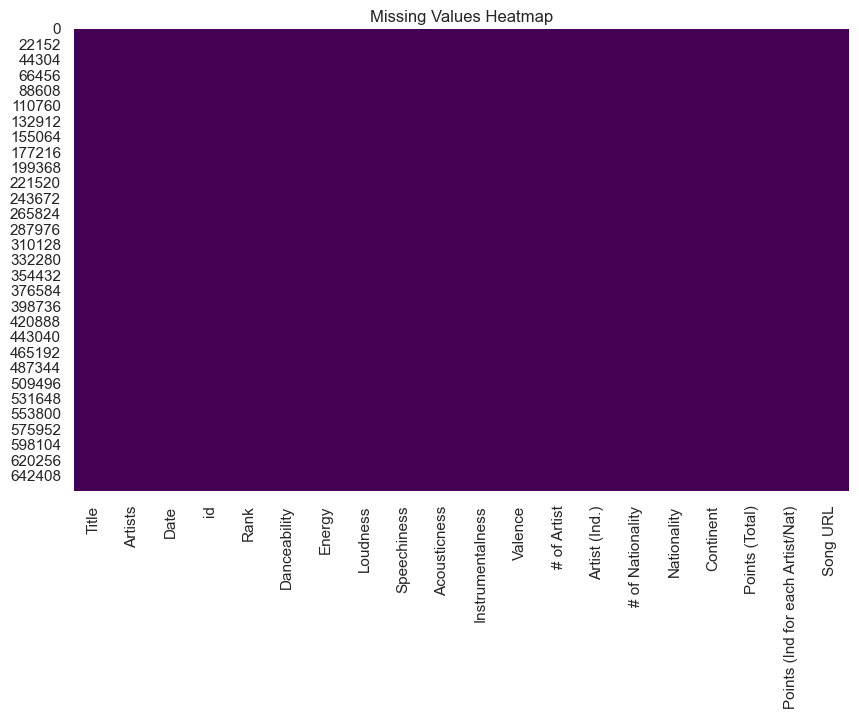
\includegraphics[width=0.5\linewidth]{Images/Data Heat Map.png}
\end{figure}

\subsubsection*{A.2 Features Distribution of Top 500 vs Bottom 500 songs}

We additionally examined the top and bottom 500 unique songs based on popularity, collected by aggregating points for ranks over six years. We used dot plots to illustrate the distribution of audio features for the two groups (Appendix B). Danceability, whose scores mostly surpass 0.5, and loudness show a concentration of higher values among the top-ranked tracks, indicating a prevalence of louder and dance-friendly songs in the Top 500. Conversely, valence and speechiness have a lesser influence on song ranking. The uniformity in the feature distributions for both the top and bottom 500 songs suggests that other factors may play a role in determining the popularity of a song.

\label{app:FEATURES500}
\begin{figure}[H]
    \centering
    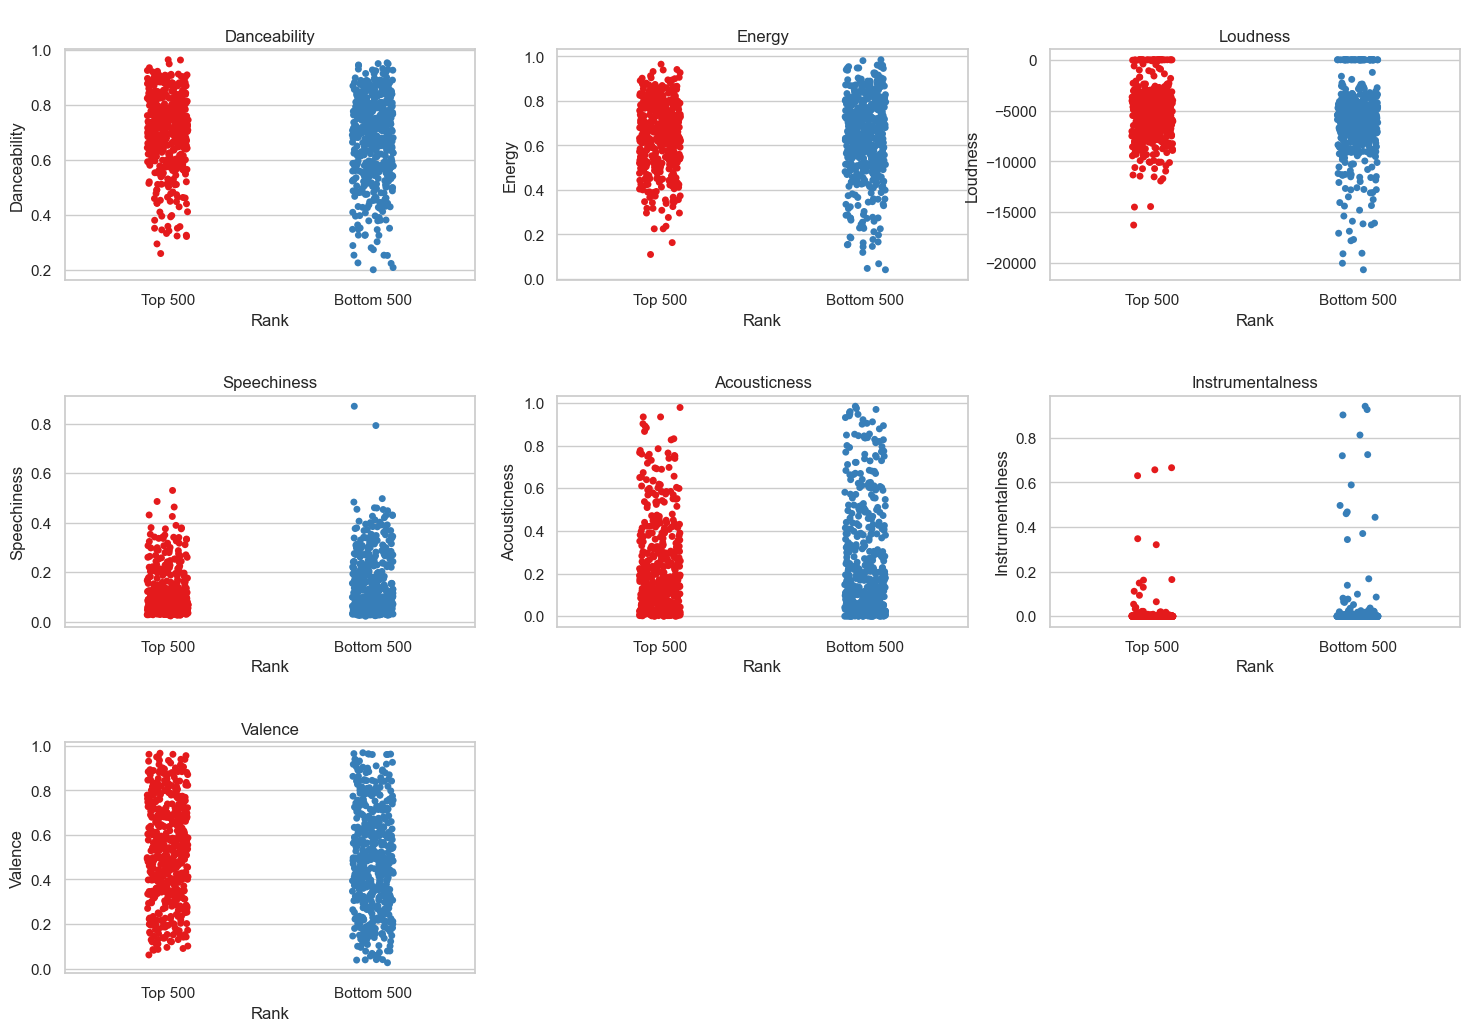
\includegraphics[width=0.8\linewidth]{Images/Features Vs Rank.png}
\end{figure}

\subsubsection*{A.3 Scatterplot to identify outliers in each feature of the transformed dataset}
\label{app:outliers-scatterplot}
\begin{figure}[H]
    \centering
    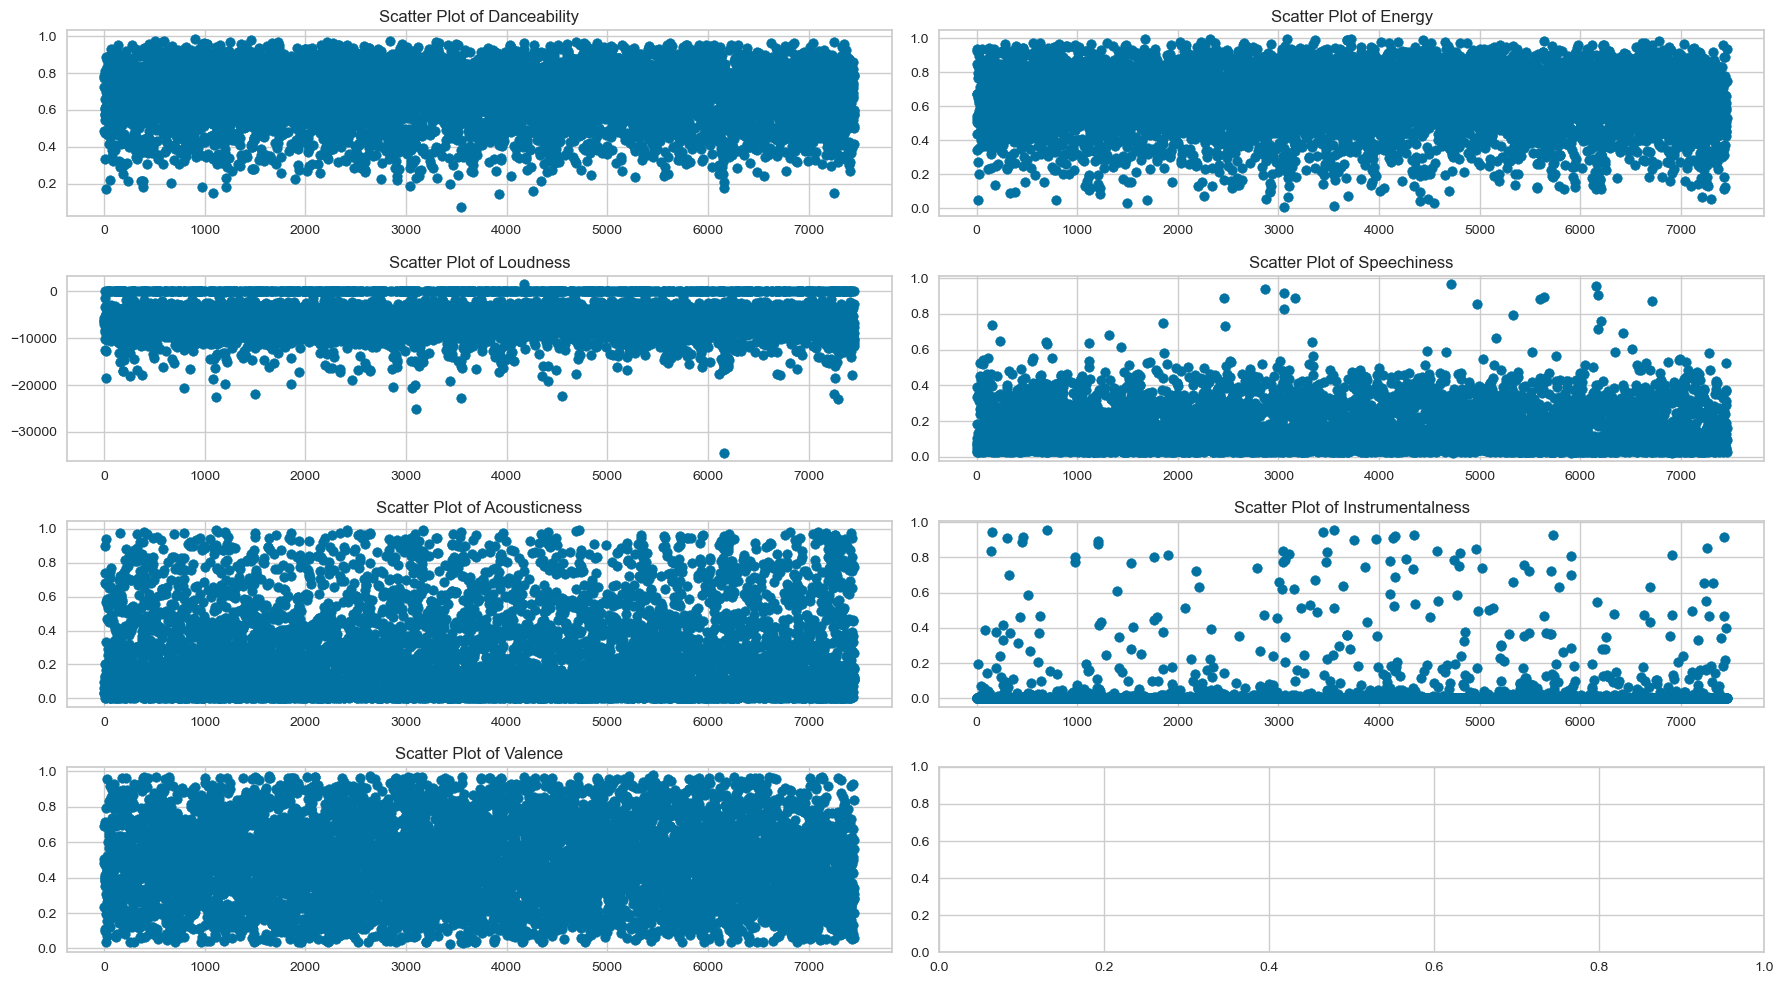
\includegraphics[width=0.7\linewidth]{Images/scatter plot for outliears.png}
\end{figure}


\section*{B. Density Based Spatial Clustering And Noise (DBSCAN)}

\label{app:DBSCAN}
\subsubsection*{B.1 K-distance Graph using nearest neighbour}
In using DBSCAN, we wanted to find the best settings for key parameters. To find the epsilon value, we looked at a K-Distance graph using the Nearest Neighbors approach to find the knee point, which helps determine the right value. From the above figure we determined the epsilon value to be 0.20
\label{app:kDist graph}
\begin{figure}[H]
    \centering
    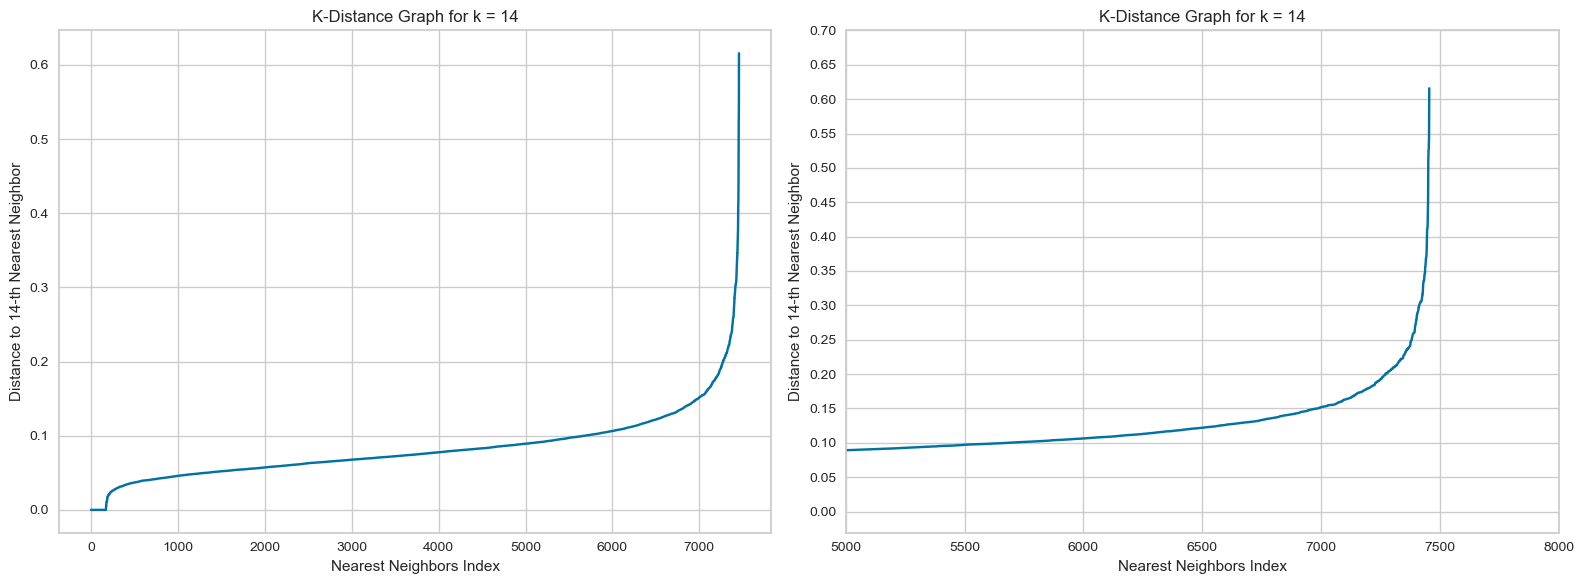
\includegraphics[width=0.8\linewidth]{Images/KL DIVERGANVE AND KNEE PLLOT.png}
\end{figure}



\subsubsection*{B.2 Estimation of no of min samples}
For another important parameter, 'min\_samples,' we used silhouette scores. From the plot above, min\_samples was determined to be 7.
\label{app:min_samples}
\begin{figure}[H]
    \centering
    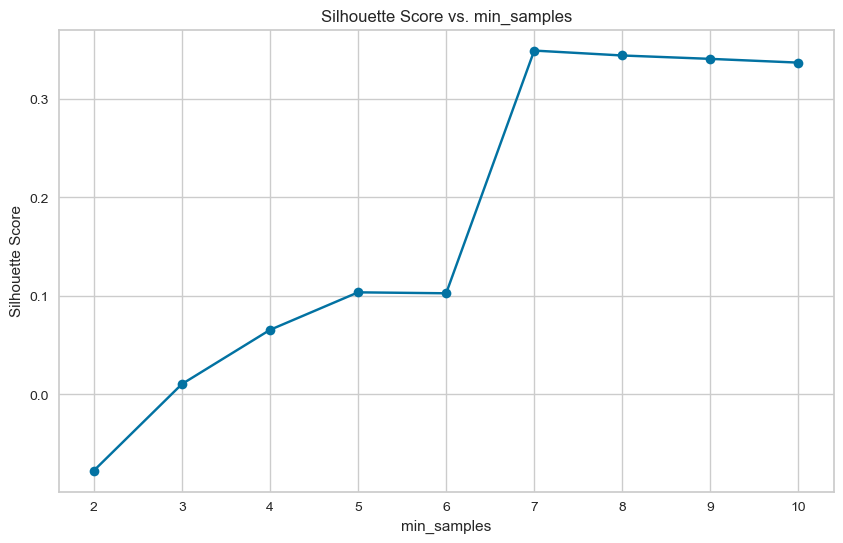
\includegraphics[width=0.7\linewidth]{Images/dbscan scores.png}
\end{figure}


\subsubsection*{B.3 Visualizing DBSCAN using PCA}
After applying DBSCAN to the dataset using epsilon and min\_samples as determined in sections B.2 and B.3, the result revealed the presence of one primary cluster(7192 data points) and identified additional data points as noise (265 noise data). The resulting clustering and noise points have been visually represented in the plot above using PCA.

\label{app:dbscan_pca}
\begin{figure}[H]
    \centering
    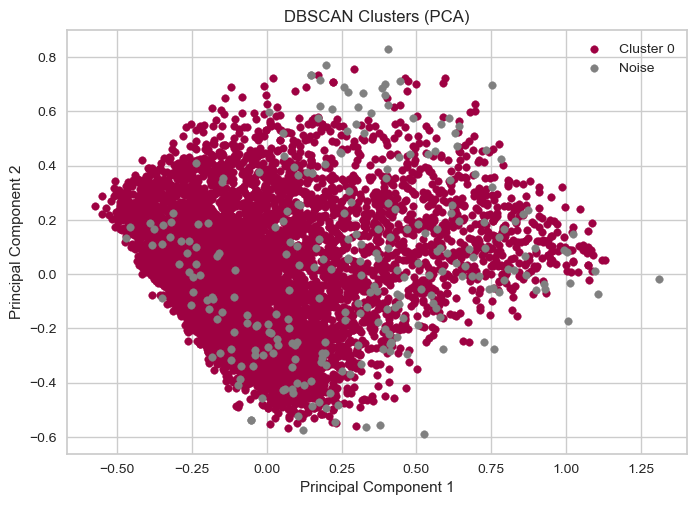
\includegraphics[width=0.9\linewidth]{Images/ddbscan plot.png}
\end{figure}




\section*{C. Dendogram for Agglomerative Clustering using Complete Linkage}
\label{app:completeLink}
\begin{figure}[H]
    \centering
    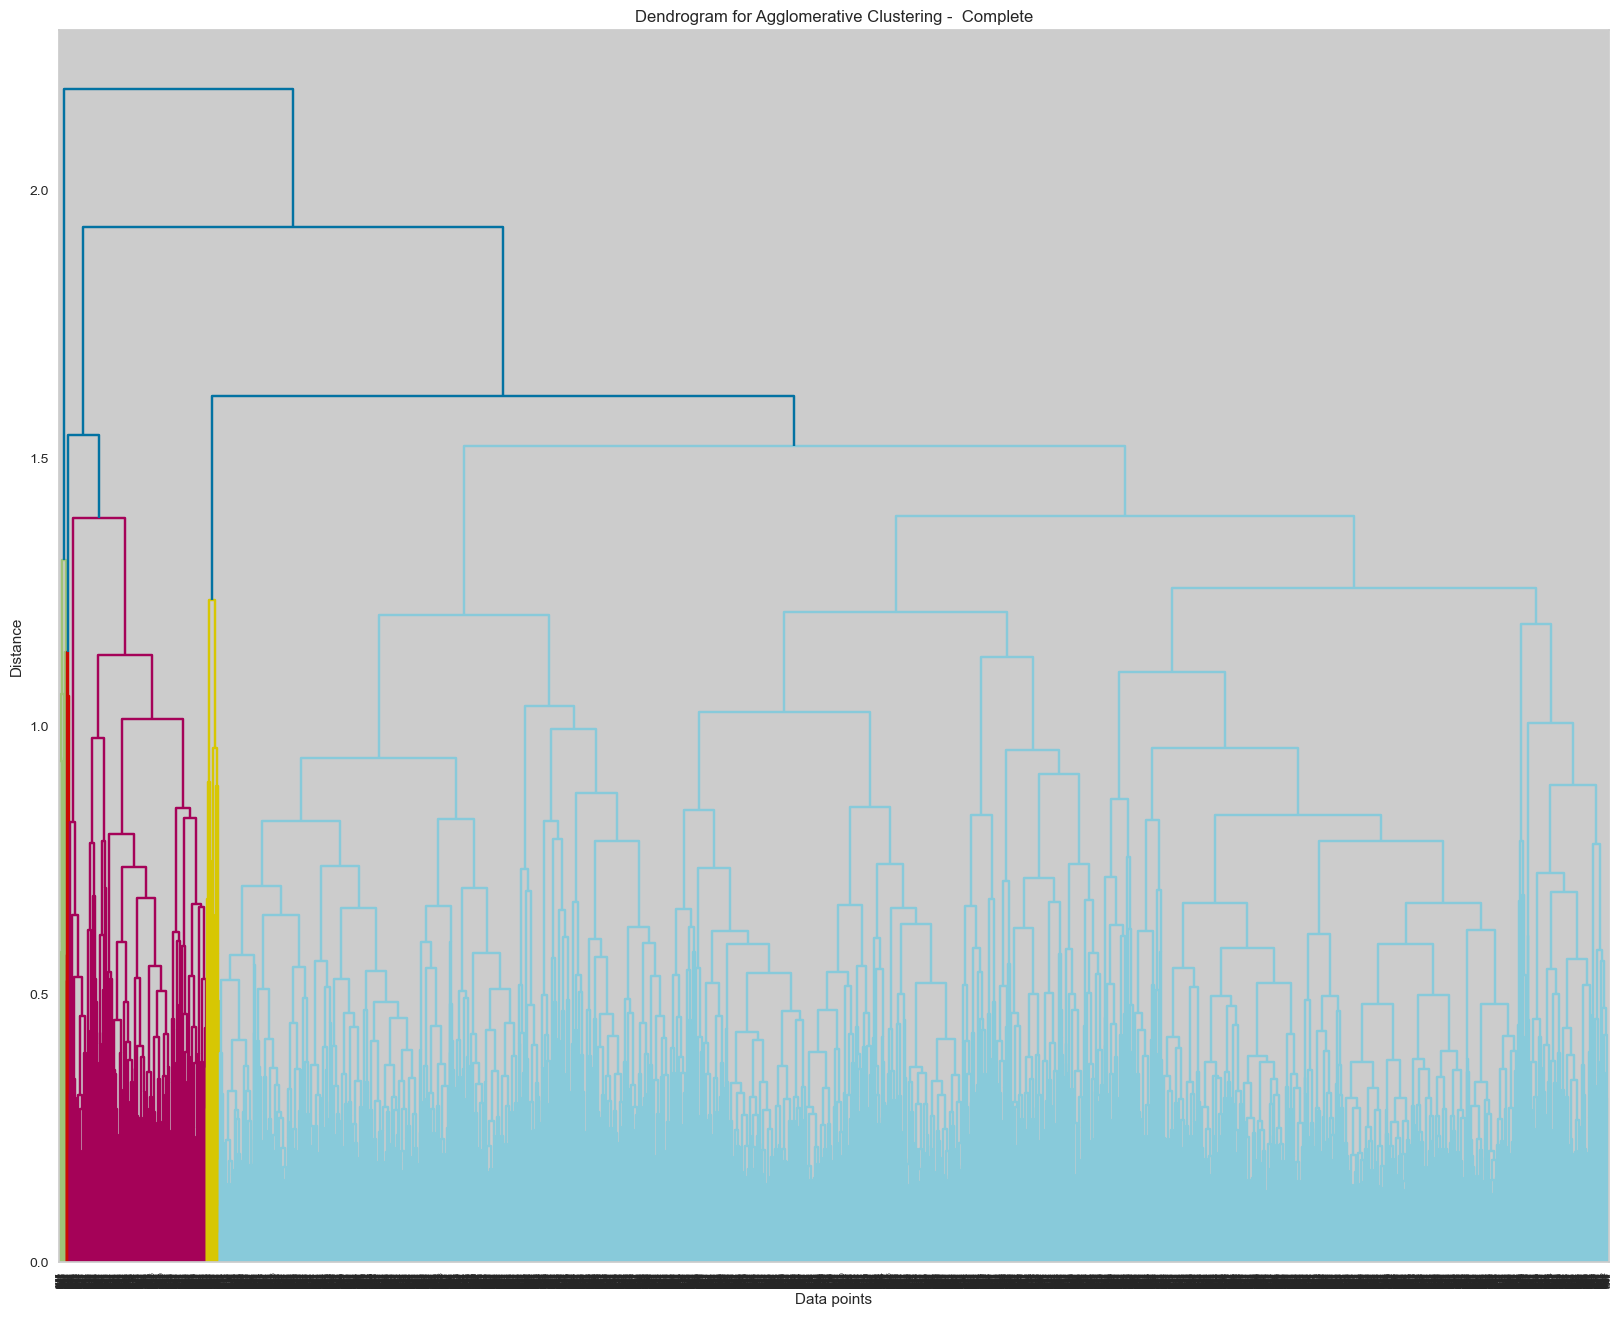
\includegraphics[width=0.7\linewidth]{Images/COMPLETE LINKAGE.png}
\end{figure}

\section*{D. Visualisation using PCA}
\subsubsection*{D.1 Amount of Variance explained by each Principal Component}
The graph shows the contribution of the first Principal Components to the variance.
\label{app:expVariance}
\begin{figure}[H]
    \centering
    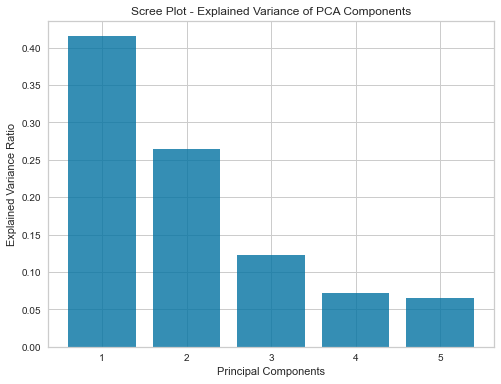
\includegraphics[width=1\linewidth]{Images/scree.png}
\end{figure}
 

\subsubsection*{D.2 Visualising K-Means clustering using PCA}
These are the Visualisations of the clusters in a scatter plot using the reduced-dimensional (PCA) with colour-coded points representing cluster assignments obtained with K-means.
\label{app:kmeans_pca}
\begin{figure}[H]
    \centering
    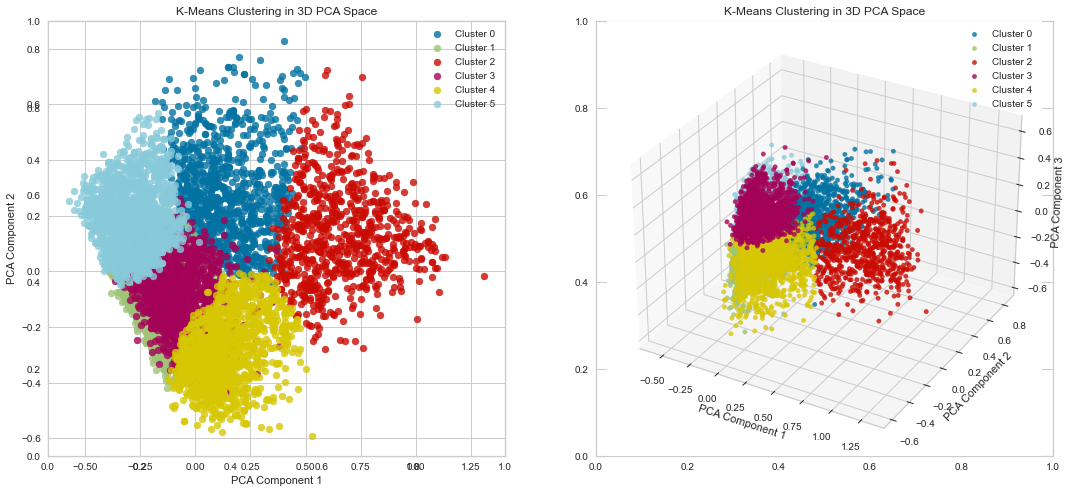
\includegraphics[width=1\linewidth]{Images/PCA K MEANS.png}
\end{figure}


\section*{E. Visualisation using t-SNE}
\label{app:TSNEPerp}
\subsubsection*{E.1 Perplexity vs KL Divergence plot}
This plot is for assessing the performance of t-SNE by finding an optimal perplexity value to preserve pairwise similarities in high-dimensional space to low-dimensional representation (indicated by the Kullback-Leibler Divergence)
\begin{figure}[H]
    \centering
    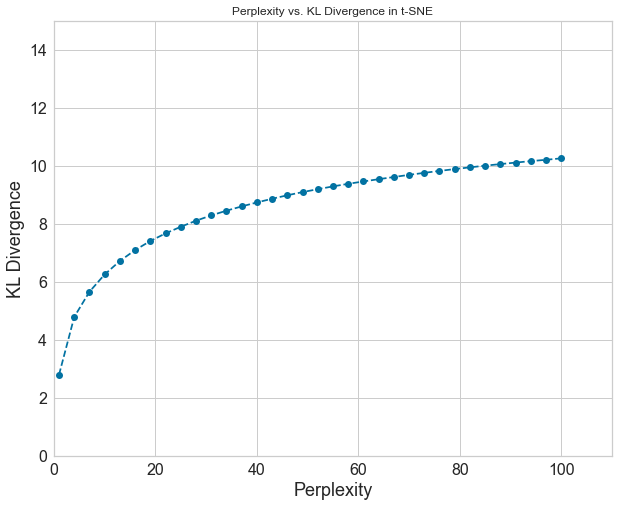
\includegraphics[width=0.76\linewidth]{Images/KL.png}
\end{figure}


\subsubsection*{E.2 K-Means clustering plots for different values of perplexity}
This plot signifies the optimal value of perplexity as 70 for the clusters to stabilize. Notably, the clusters hardly change after the optimal value is reached.
\begin{figure}[H]
    \centering
    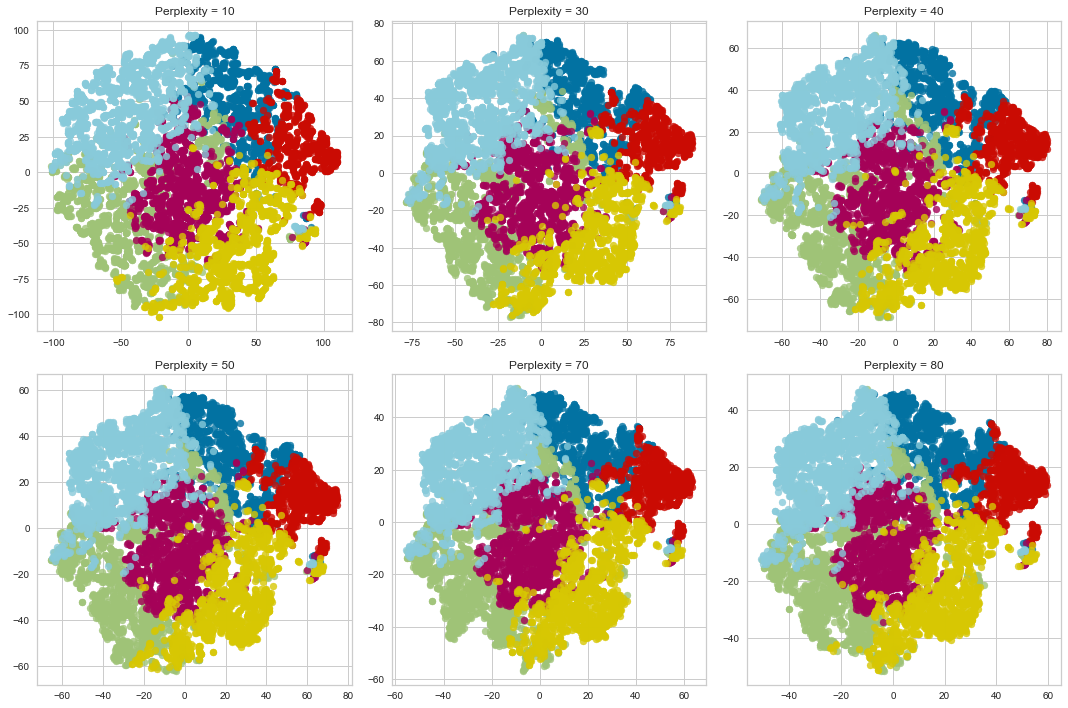
\includegraphics[width=0.88\linewidth]{Images/TSNE.png}
\end{figure}


\section*{F. Cluster Profiling: Interpreting the qualitative nature of songs in each cluster}
\textbf{Cluster 0}: Natural and acoustic songs with positive, engaging lyrics and diverse emotional essence with a positive ring to it

\textbf{Cluster 1}: Songs have high energy and loudness with a good blend of vocals and music. They have a broad palette for a range of emotions. 

\textbf{Cluster 2}: Songs that are soft and soothing, composed of acoustics and instrumentals, but whose lyrics seem to be on the less happy side.

\textbf{Cluster 3}: Songs belonging to this cluster are loud, energizing and positive in expression. They are mostly lyrical, like rap, and induce a lively atmosphere conducive to dancing to their beats. 

\textbf{Cluster 4}: Energetic songs with high beats but gloomy lyrics and fewer acoustics and instrumentals.

\textbf{Cluster 5}: Danceable, loud and high energy tracks with minimal instrumentals. These songs too, have lyrics that invoke highly positive emotions.

 
The mean levels of Danceability, energy and loudness are high for every cluster except cluster 2. The most groovy songs can be found in Clusters 3 and 5 while high energy songs mostly belong to clusters 1 and 5. Cluster 3 exhibits a high value of speechiness indicating the presence of more lyrical songs like rap. The gloomy songs in Cluster 2 have exceptionally high acousticness and instrumentalness, compared to the other clusters. Listening to songs from clusters 0 and 5 invoke highly positive emotions, while songs in clusters 1 and 4 induce relatively negative feelings.

\label{app:Cluster_profile}
\begin{figure}[H]
    \centering
    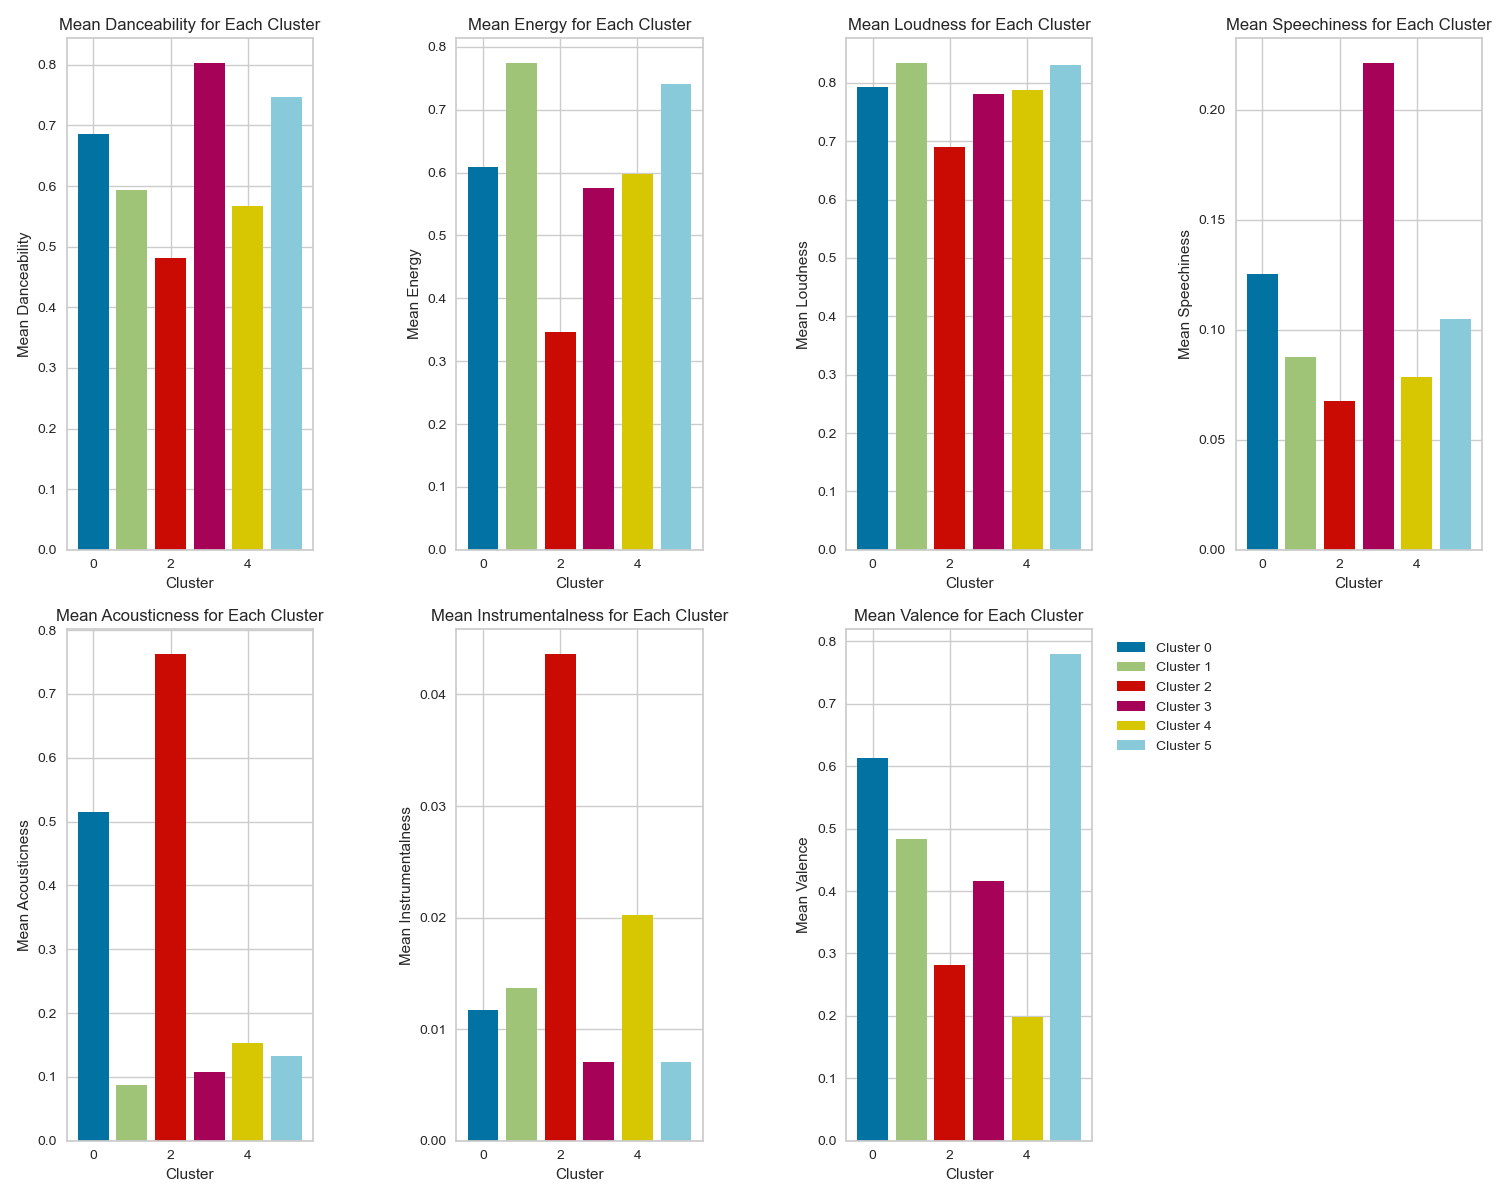
\includegraphics[width=1\linewidth]{Images/mean_values_cluster.png}
\end{figure}

Mean value analysis helps us to indicate that our recommender system shows a stable and dependable pattern in capturing the user's preferences and aligning the suggested songs with appropriate clusters. The feature values of the recommended song are comparable to the mean attribute values of all the songs specified by the user in his input (single song/playlist).
\clearpage
\section*{G Plots of Similarity Measures for Recommender System}

The mean values of the features for recommended songs, which were suggested using Euclidean, Manhattan, and Cosine metrics, were plotted alongside their respective feature values of the songs inputted by User 1 and User 2. The plots are shown below in sections G.1, G.2, and G.3.




\label{app:RECOM_MEAN_PLOT}
\subsubsection*{G.1 Similarity Metric - Manhattan Distance}
\label{app:Manhattan}
\begin{figure}[H]
    \centering
    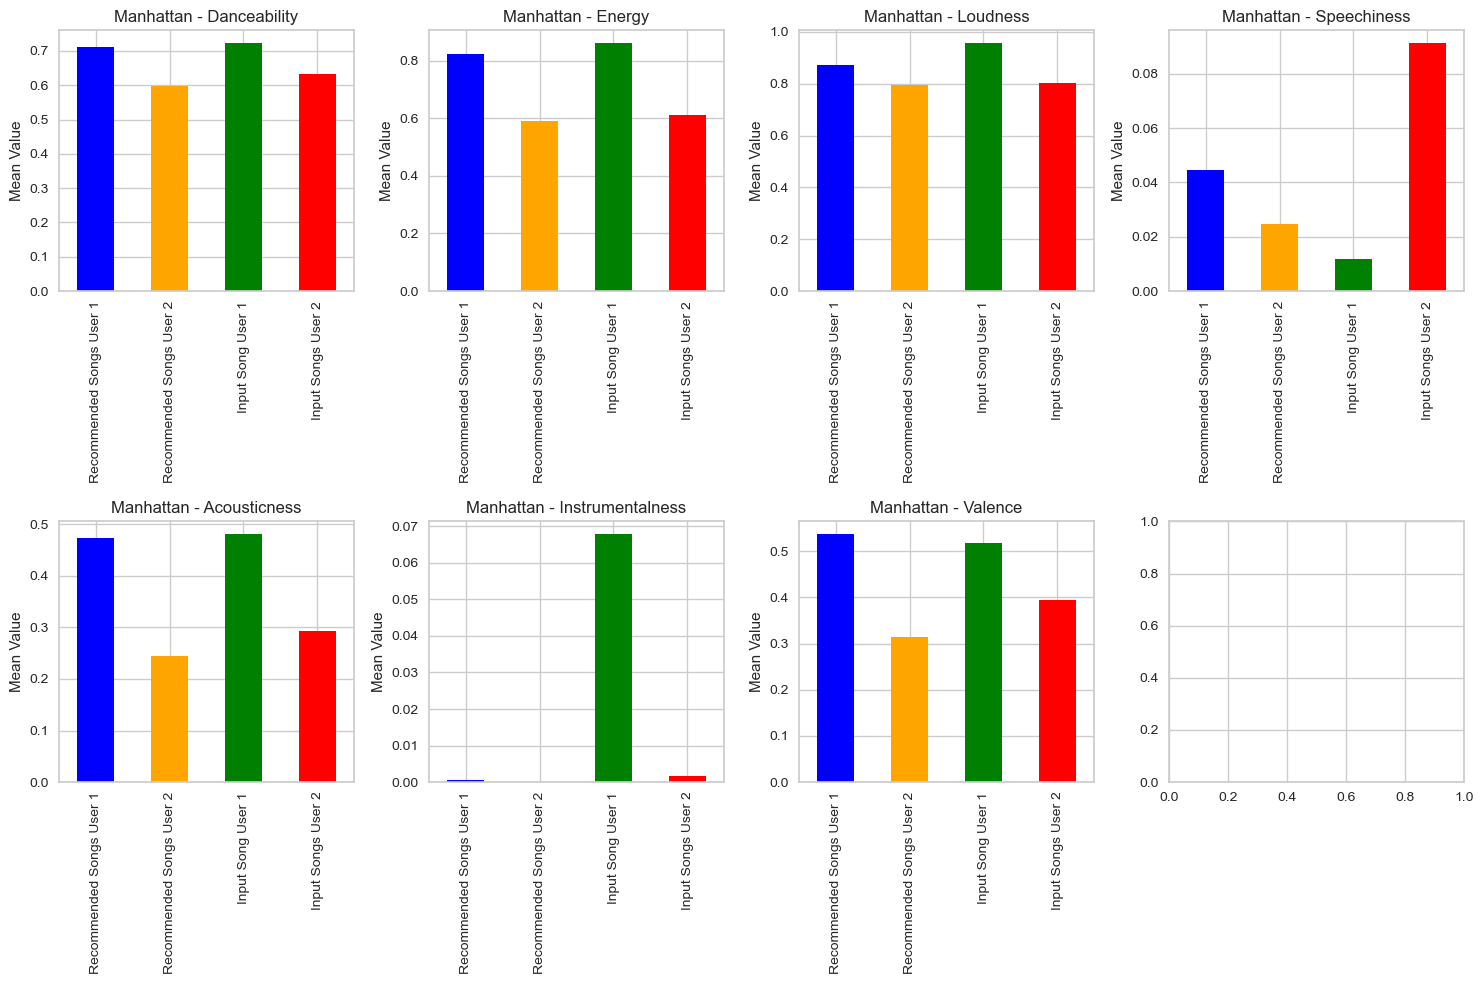
\includegraphics[width=0.9\linewidth]{Images/manhattan_mean_values.png}
\end{figure}
\subsubsection*{G.2 Similarity Metric - Euclidean Distance}
\label{app:Euclidean}
\begin{figure}[H]
    \centering
    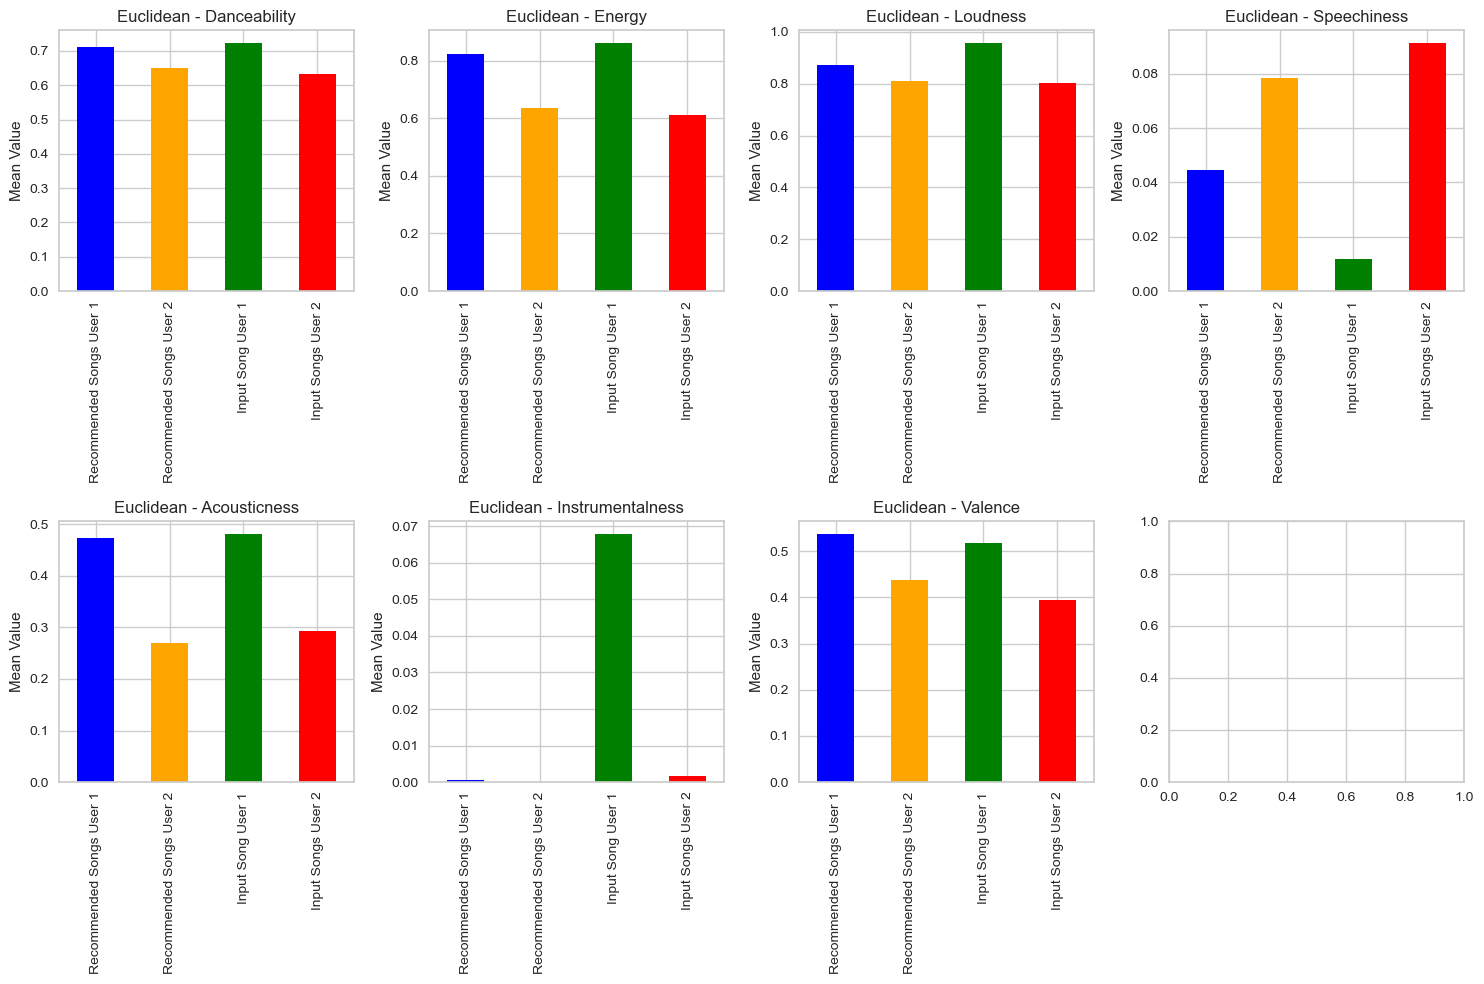
\includegraphics[width=0.9\linewidth]{Images/Euclidean_mean_values.png}
\end{figure}
\subsubsection*{G.3 Cosine Similarity}
\label{app:CosineSim}
\begin{figure}[H]
    \centering
    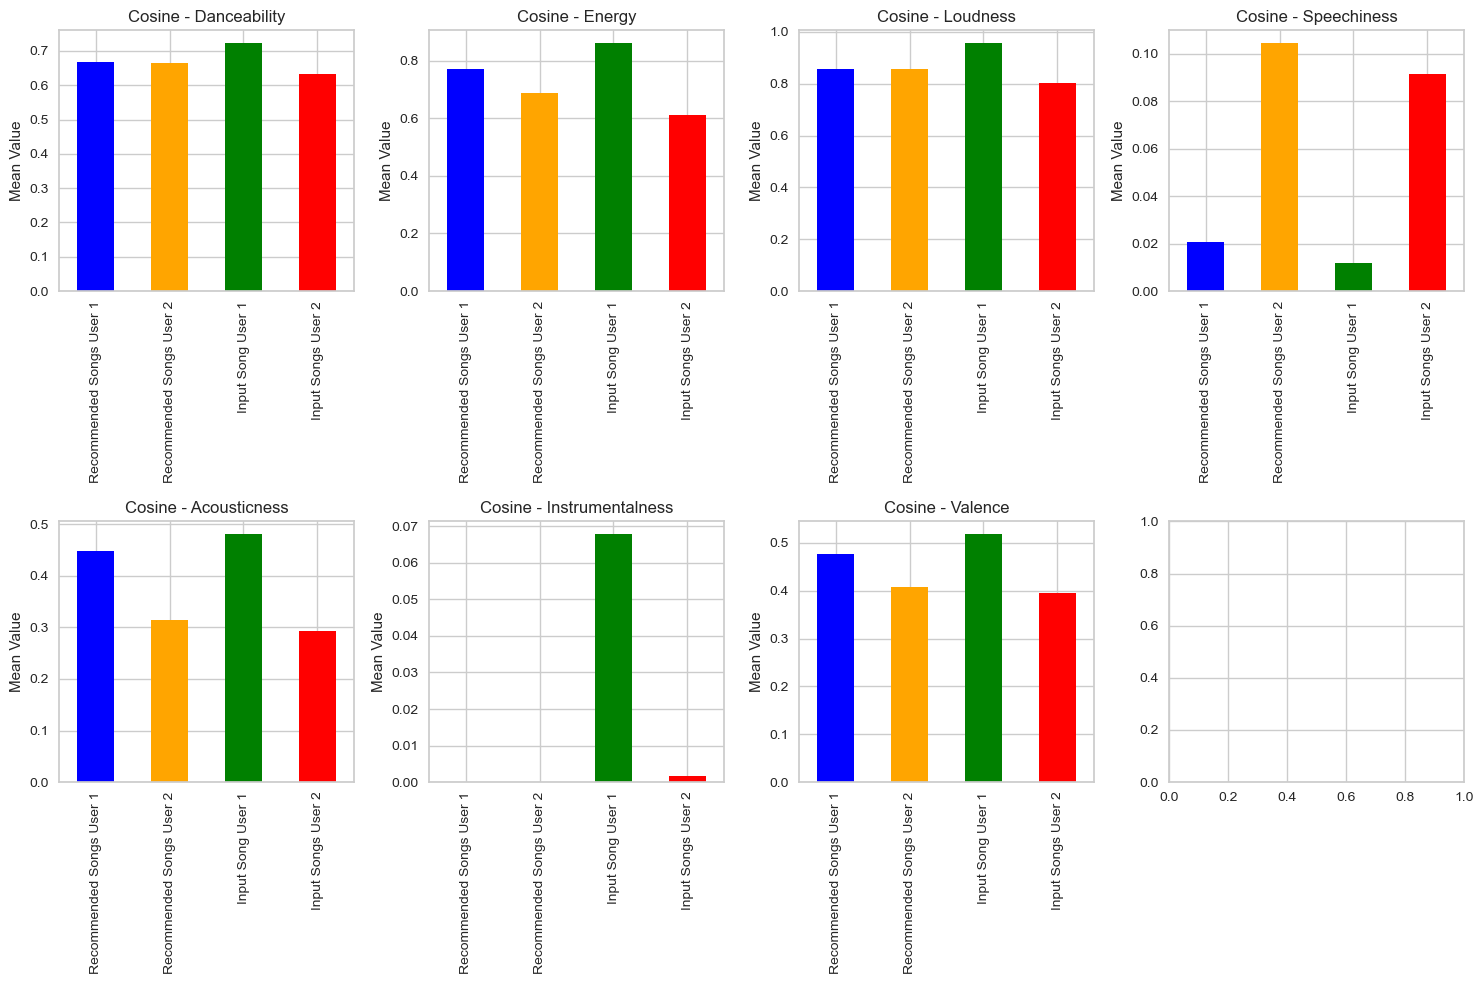
\includegraphics[width=0.9\linewidth]{Images/Cosine_mean_values.png}
\end{figure}

\section*{H. User Inputs and their corresponding attribute means}
\label{app:RecSysOP}
%\centering


% We used Box Plot to confirm the presence of outliers for each feature. Data points lying beyond the acceptable range [(Q1 - 1.5 * IQR) , (Q3 + 1.5 * IQR)], where IQR = (Q3 - Q1), were marked as outliers and removed from the data as they could significantly impact clustering results.

% As mentioned earlier in the report, we determined the perplexity using the KL Divergence plot, resulting in a perplexity value of 80. Subsequently, we generated clustering plots for three distinct perplexity ranges: before, at, and after perplexity 80. The plots clearly indicate that clustering stabilizes after reaching a perplexity of 80, with minimal changes observed in the clustering structure. 





\begin{table}[H]
\centering
\begin{tabular}{lc}
\toprule
\textbf{Song Title}           & \textbf{Cluster} \\ \hline
Smoking on my Ex Pack    & 4       \\
Black SpiderMan          & 1       \\
Always                   & 2       \\
Snow On Tha Bluff        & 2       \\
Kiss Me More (feat. SZA) & 5       \\
Sweat                    & 4       \\
fuck, i'm lonely         & 0       \\
WTF Do I Know            & 1       \\
Boys Will Be Boys        & 0       \\ 
Top Down On Da WF        & 4       \\ \hline
\end{tabular}%
\\[1ex]
\caption{Songs in User 2's input playlist and the clusters they belong to}
\label{tab:my-table1}
\end{table}

\begin{table}[H]
\centering
\begin{tabular}{lcc}
\toprule
\textbf{Song Attribute} & \textbf{User 1} & \textbf{User 2} \\ \hline
Danceability            & 0.723684        & 0.634101        \\ 
Energy                  & 0.861756        & 0.612210        \\ 
Loudness                & 0.957925        & 0.800994        \\ 
Speechiness             & 0.011653        & 0.091419        \\ 
Acousticness            & 0.481891        & 0.294064        \\ 
Instrumentalness        & 0.067992        & 0.001674        \\ 
Valence                 & 0.518908        & 0.394223        \\ \hline
\end{tabular}
\\[1ex]
\caption{Mean value of features for User 1 \& 2 Input}
\label{tab:my-table2}
\end{table}


\section*{I. Description and Formulae of Clustering Evaluation Metrics}

The \textbf{Silhouette score} considers both cohesion (intra-cluster similarity) and separation (inter-cluster distance). It ranges from [-1, 1], where a high value indicates that the object is well-matched to its own cluster and distinguishable from neighbouring clusters. If a(i) represents the average distance of a point to other points in the same cluster and b(i) represents the average distance of a point to points in the nearest neighboring cluster, the Silhouette score is calculated by the formula below:
\begin{figure}[H]
    \centering
    
\includegraphics[width=0.4\linewidth]{Images/silhouette.png}
\end{figure}

The \textbf{Davies-Bouldin index} is defined as the average similarity measure of each cluster with its most similar cluster, where similarity is the ratio of within-cluster distances to between-cluster distances. The minimum score is zero, with lower values indicating better clustering. The Davies-Bouldin score can be computed using the formula below:

\begin{figure}[H]
    \centering
    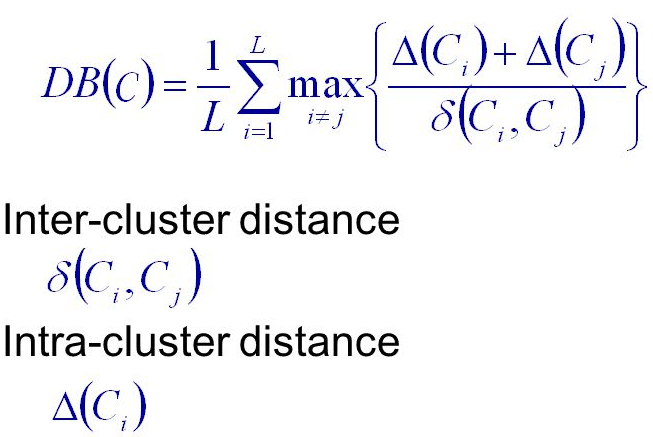
\includegraphics[width=0.5\linewidth]{Images/DB score.png}
\end{figure}

The \textbf{Calinski-Harabasz index} or the variance-ratio criterion is the ratio of the sum of between-clusters dispersion and of inter-cluster dispersion for all clusters. The index assesses how well-separated clusters are by comparing the dispersion within clusters to the dispersion between clusters. The higher the score, the better is the performance of the clustering algorithm. It is calculated using the formula below:

\begin{figure}[H]
    \centering
    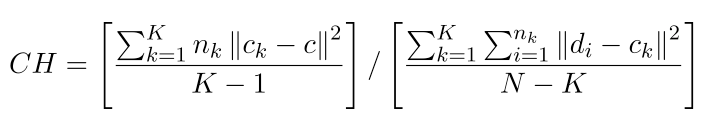
\includegraphics[width=0.8\linewidth]{Images/calinski_harabasz.png}
\end{figure}

\clearpage
\section*{J. Similarity Metrics for Content Based Filtering for Recommendation Systems}

\textbf{Manhattan Distance} computes the sum of the absolute differences between their coordinates. It represents the sum of the shortest paths that could be taken between two points along orthogonal axes. It is calculated using the formula below:

\begin{figure}[H]
    \centering
    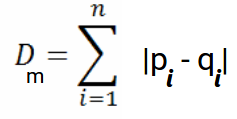
\includegraphics[width=0.25\linewidth]{Images/manhattan.png}
\end{figure}

\textbf{Euclidean Distance}, which is given by the formula below, represents the straight-line distance and quantifies the amount of similarity or dissimilarity between points in a multidimensional space

\begin{figure}[H]
    \centering
    
\includegraphics[width=0.4\linewidth]{Images/euclidean.png}
\end{figure}

The interpretation in terms of similarity is same for both the metrics. The closer the points are in the high dimensional space, lesser is the distance and greater is the similarity. Graphically, the difference between the two metrics can be understood from the figure below.

\begin{figure}[H]
    \centering
    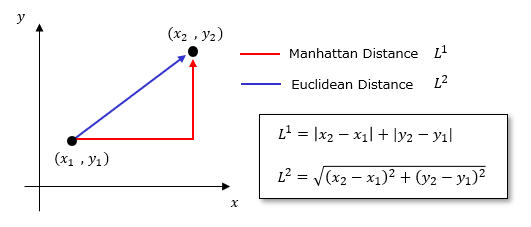
\includegraphics[width=0.7\linewidth]{Images/man euc graphical.png}
\end{figure}

\textbf{Cosine Similarity} quantifies the similarity between vectors in a multidimensional space by evaluating the cosine of the angle between the them. It indicates how closely the vectors are pointing in the same direction by computing the dot product of the respective vector norms, using the formula:

\begin{figure}[H]
    \centering
    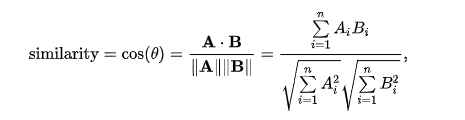
\includegraphics[width=0.7\linewidth]{Images/cosine-similarity.png}
\end{figure}

The interpretation of cosine similarity can be understood from the figure below:

\begin{figure}[H]
    \centering
    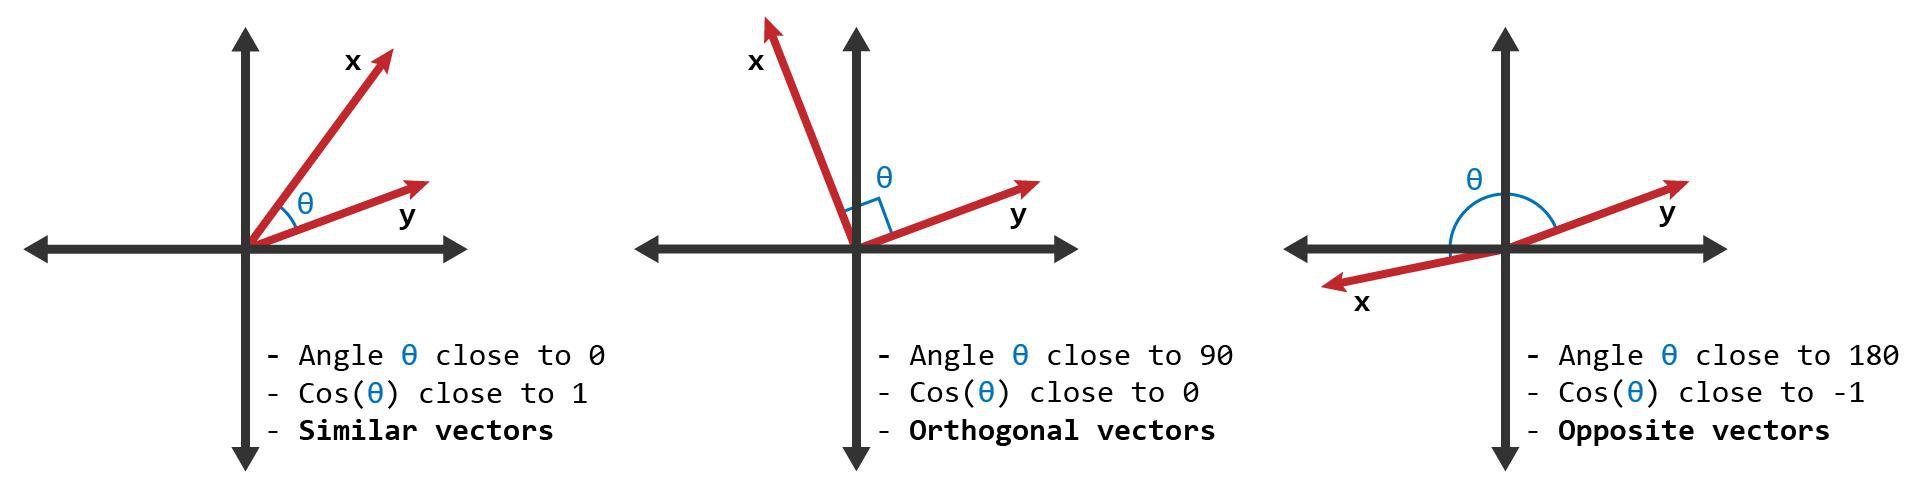
\includegraphics[width=0.7\linewidth]{Images/cos sim.jpg}
\end{figure}

\end{document}



%%% Local Variables:
%%% mode: latex
%%% TeX-master: t
%%% End:
